\documentclass[a4paper,12pt]{report}
\usepackage{styles/fbe_tez}
\usepackage[utf8x]{inputenc} % To use Unicode (e.g. Turkish) characters
\renewcommand{\labelenumi}{(\roman{enumi})}
\usepackage{amsmath, amsthm, amssymb}
\usepackage[bottom]{footmisc}
\usepackage{cite}
\usepackage{url}
\usepackage{graphicx}
\usepackage{longtable}
\graphicspath{{figures/}{images/}}

\usepackage{multirow}
\usepackage{subfigure}
\usepackage{algorithm}
\usepackage{algorithmic}
\usepackage{float}

\begin{document}

% Title Page
\title{CMPE 492 \\ Nounce: Language Platform for Phonetic Analysis \& Pronunciation Assessment}
\author{
Ümit Can Evleksiz \\
Ömer Faruk Bayram \\ \\
Advisor: \\
Prof. Lale Akarun \\
Prof. Murat Saraçlar
}
\date{}
\maketitle{}
\pagenumbering{roman}
\tableofcontents

\chapter{INTRODUCTION}
\pagenumbering{arabic}

\section{Broad Impact}

\subsection{Learning Impact}

Nounce is a web-based pronunciation assessment application that provides learners with practical how-to knowledge for speaking standard English, focusing on pronunciation accuracy and clarity. By introducing users to the International Phonetic Alphabet (IPA) and phonetic concepts, the system builds domain familiarity, enabling learners to discuss and understand sound units systematically. The platform incorporates gamification elements and provides fast, friendly feedback to create a safe learning environment where users can practice without fear of judgment.

It is important to note that the objective is not to replace human-to-human interactions in language learning, but rather to provide accessible tools for individuals who may lack access to human tutors, native speaker friends, or formal language education resources. The system serves as a supplementary tool that empowers self-directed learning while acknowledging the irreplaceable value of human interaction in language acquisition.

\subsection{Academic Impact}

This project contributes to the academic community by demonstrating the practical application of fine-tuning deep learning models for specialized phonetic transcription tasks. The work combines core signal processing techniques with modern machine learning approaches, integrating multiple moving parts including audio preprocessing, phonetic transcription, forced alignment, and pronunciation assessment into a cohesive full-stack application. The system showcases how research-grade models can be adapted and deployed in real-world educational contexts, providing a reference implementation for similar pronunciation assessment systems.

\section{Ethical Considerations}

\subsection{User Speech Data}

The system handles sensitive user speech data, which raises important privacy and usage concerns. Audio recordings are used for inference during pronunciation assessment, but users must explicitly opt-in for any potential use of their data in model fine-tuning, voice cloning, or correct pronunciation generation features. Clear consent mechanisms and transparent data usage policies are essential to protect user privacy and maintain trust.

\subsection{Prescriptive Approach in Linguistics}

The application focuses on US English pronunciation, which may appear prescriptive. However, it is crucial to emphasize that all dialects, accents, and language variants are linguistically valid. US English is chosen not to minimize or devalue other accents, but because it is widely adopted and in high demand globally, particularly in professional and academic contexts. The system aims to improve comprehensibility and communication effectiveness rather than eliminate linguistic diversity. Users are encouraged to understand that accent reduction is optional and that the primary goal is clear communication, not accent elimination.

\subsection{Monetization and Accessibility}

Commercialization of educational technology raises concerns about potentially gatekeeping education from economically disadvantaged populations. While the system may include premium features or subscription models, careful consideration must be given to ensuring that core pronunciation assessment capabilities remain accessible. Free tiers, educational discounts, and open-source components can help mitigate barriers to access, ensuring that pronunciation learning tools do not become exclusive to those who can afford them.

\chapter{PROJECT DEFINITION AND PLANNING}
\section{Project Definition}
This project develops Nounce, a web-based application to assist English language learners in improving pronunciation through automated speech analysis and personalized feedback. The system enables users to record speech, receive detailed pronunciation assessments, and gain insights into English phonology.

Core functionality includes: (i) capturing and processing user speech recordings, (ii) analyzing pronunciation accuracy at the phonetic level using machine learning models, (iii) comparing actual pronunciation against target acoustic patterns, and (iv) providing educational guidance on English phonology.

The system focuses on English with US accent (potentially including UK), with initial development targeting Turkish-native English speakers. Future milestones will leverage users' native language to better detect phonetic units. The application is designed to be accessible and pedagogically sound, emphasizing comprehensibility over accent elimination.

\subsection{Relationship to the CMPE491 Prototype}
\label{sec:v1-vs-v2}

Nounce builds directly on a prototype developed for CMPE491. That first version established the end-to-end recording-to-feedback concept, but several of its components proved unreliable or pedagogically thin. The present work (CMPE492) reworks the system around two themes---\emph{reliability} and \emph{deviation-awareness}---and the improvements over the prototype are detailed in the relevant sections rather than enumerated here. In brief: forced alignment moves from the Montreal Forced Aligner to POWSM's own CTC alignment, giving a single consistent phone inventory and real frame-level timestamps (Chapter~6); synthesized text-to-speech reference audio is retired in favour of human native recordings in General American and Received Pronunciation; an audio-quality stage now detects no-speech, noisy, and wrong-sentence input and abstains rather than returning a misleading score; the phone-level difference and the learner-facing feedback are computed over articulatory feature vectors instead of exact-match string comparison, so they reflect \emph{how far} a produced phone is from the target; and the interface adds per-phone playback with synchronized highlighting and goodness-of-pronunciation colouring. Most significantly, where the prototype shipped without any formal evaluation, this version introduces dedicated validation sets, a cross-dataset fine-tuning study, and a human-judgment correlation analysis (Section~\ref{sec:finetuning-results}). The through-line is a shift from a transcribe-and-compare prototype to an evaluated assessment system that detects and explains pronunciation deviations.

\section{Project Planning}
\subsection{Project Time and Resource Estimation}
The project is developed as a two-person team effort with the following resource allocation:

\textbf{Time Commitment:}
\begin{itemize}
    \item Development time: ~15 hours per week per team member
    \item Project duration: Two academic semesters (CMPE 491 + CMPE 492)
    \item Total estimated effort: ~360 hours per member
\end{itemize}

\textbf{Infrastructure Costs:}
\begin{itemize}
    \item Full-stack server hosting: \$5 per month
    \item Serverless PostgreSQL database: \$5 per month
    \item Serverless GPU for ML job queue: \$20-30 per month (moderate user activity)
    \item Total monthly infrastructure cost: \$30-40 per month
\end{itemize}

\textbf{Additional Resources:}
\begin{itemize}
    \item Development tools and frameworks (open-source)
    \item ML model training and evaluation datasets
    \item Audio processing libraries and APIs
\end{itemize}

\subsection{Success Criteria}
The project will be considered successful upon achieving the following objectives:

\textbf{Technical Requirements:}
\begin{itemize}
    \item Full-stack secure web application with authentication and authorization
    \item System uptime of 99\% or higher
    \item Acoustic ML model producing accurate phonetic-level transcriptions independent of prosodic variations
    \item Difference algorithm comparing actual pronunciation against target patterns with actionable feedback
    \item Scalable architecture supporting concurrent sessions and asynchronous audio processing
\end{itemize}

\textbf{User Experience Requirements:}
\begin{itemize}
    \item Industry-grade UI/UX following modern web standards
    \item Intuitive workflow for recording, uploading, and reviewing feedback
    \item Clear presentation of pronunciation analysis results
    \item Responsive design supporting multiple devices
    \item Accessible interface adhering to web accessibility guidelines
\end{itemize}

\textbf{Functional Requirements:}
\begin{itemize}
    \item Accurate real-time or near-real-time pronunciation assessment
    \item Educational content integration for English phonology
    \item Progress tracking and historical analysis
    \item Support for multiple audio formats and quality levels
\end{itemize}

\subsection{Risk Analysis}
Several risks have been identified that may impact project success:

\textbf{Technical Risks:}
\begin{itemize}
    \item \textbf{ML Model Performance:} The machine learning model may not achieve desired accuracy, particularly with low-quality audio, background noise, or non-standard accents. Mitigation includes extensive training on diverse datasets, robust preprocessing, and fallback mechanisms for low-confidence predictions.
    \item \textbf{Audio Quality Variability:} Users may submit recordings with varying quality, device capabilities, and environmental conditions. The system must handle this through adaptive preprocessing and quality assessment.
    \item \textbf{Computational Resource Constraints:} Processing requirements may strain serverless GPU resources during peak usage. Load balancing, queue management, and resource scaling will address this.
    \item \textbf{Integration Complexity:} Coordinating multiple system components may introduce integration challenges. Comprehensive testing and modular architecture will mitigate these risks.
\end{itemize}

\textbf{Pedagogical and Ethical Risks:}
\begin{itemize}
    \item \textbf{Language and Accent Limitations:} The application focuses on English with US accent (potentially UK). Other languages are not supported. Initial development targets Turkish-native English speakers, with future milestones leveraging native language for better phonetic detection. This limitation must be clearly communicated to users to avoid misconceptions about supported languages and accents.
    \item \textbf{Overly Prescriptive Approach:} The system may promote misconceptions about a single "correct" pronunciation, marginalizing linguistic variation. This is addressed by emphasizing comprehensibility over accent matching, acknowledging linguistic diversity, and transparently communicating system limitations.
    \item \textbf{User Expectations vs. Reality:} Users may have unrealistic expectations about pronunciation transformation. Clear communication about the tool's purpose as a learning aid is essential.
    \item \textbf{Data Privacy and Security:} Handling sensitive user audio data requires robust security measures and clear privacy policies. Users must explicitly opt-in for any use of their data in model fine-tuning, voice cloning, or pronunciation generation. Compliance with data protection regulations will be prioritized.
    \item \textbf{Accessibility and Monetization:} Commercial features may create barriers for economically disadvantaged users. Free tiers and educational discounts should be considered to ensure accessibility.
\end{itemize}

\textbf{Project Management Risks:}
\begin{itemize}
    \item \textbf{Coordination Overhead:} With two team members working on different components, ensuring consistent integration and avoiding conflicting changes requires regular communication and code review.
    \item \textbf{Scope Creep:} The project may expand beyond initial scope. Potential scope creep includes voice cloning and generating correct pronunciation using the user's voice, which are explicitly out of scope. A clear feature prioritization framework and milestone-based development approach will maintain focus.
\end{itemize}

\subsection{Team Work}
This project is developed as a two-person team effort with complementary responsibilities:

\begin{itemize}
    \item \textbf{Ümit Can Evleksiz:} Full-stack web application development, ML pipeline integration (assessment and IPA generation endpoints), audio preprocessing, deployment infrastructure, database design, and CI/CD pipelines.
    \item \textbf{Ömer Faruk Bayram:} POWSM-CTC model evaluation and experiments, admin analytics dashboard development, and signal processing research.
\end{itemize}

Both team members contributed to documentation, testing, and project planning.

\chapter{RELATED WORK}

\section{Speech Foundation Models and Phonetic Transcription}

Several open-source deep learning models are available for phonetic transcription. Wav2Vec 2.0 \cite{baevski2020wav2vec} and WavLM \cite{chen2022wavlm} provide self-supervised speech representations that can be fine-tuned for phonetic recognition, though they require significant adaptation. For this application, POWSM (Phonetic Open Whisper-Style Speech Model) \cite{powsm} is best suited, as it is specifically engineered for phonetic transcription with textual transcription context. The model is open to fine-tuning, which is valuable for adapting to Turkish-native English speakers. Connectionist Temporal Classification (CTC) \cite{graves2006connectionist} is commonly used for sequence alignment in phonetic transcription tasks.

\section{CTC-Based Speech Models}

Connectionist Temporal Classification (CTC) \cite{graves2006connectionist} is widely used for sequence alignment in speech processing. OWSM-CTC \cite{owsmctc} is an encoder-only variant of the Open Whisper-Style Speech Model that uses CTC loss instead of an encoder-decoder architecture. With 1 billion parameters trained on 180,000 hours of multilingual speech data, OWSM-CTC achieves 3--4$\times$ faster inference than its encoder-decoder counterpart while supporting multilingual ASR, speech translation, and language identification. The non-autoregressive nature of CTC models makes them attractive for real-time applications; however, the lack of a decoder limits their ability to perform text-conditioned tasks such as Grapheme-to-Phoneme (G2P) conversion, which is essential for pronunciation assessment pipelines.

\section{Forced Alignment and Assessment}

The Montreal Forced Aligner (MFA) \cite{mcauliffe2017montreal} is an industry-standard tool for phoneme-level time alignment, supporting English out-of-the-box, and was used in the CMPE491 prototype. In the present work, however, time alignment is performed with POWSM's own CTC forced alignment rather than MFA, which keeps recognition and alignment on a single phone inventory (Chapter~6). Pronunciation assessment employs metrics such as Phoneme Error Rate (PER) and goodness of pronunciation (GOP) scores \cite{witt2000phone} to evaluate speech quality.

\section{L2 Speech Corpora and the Annotation Gap}
\label{sec:data-gap}

A model that \emph{detects} mispronunciations must be trained on what the learner actually \emph{produced}, not on the dictionary form of the target word---otherwise it learns to normalize deviations away rather than surface them. This bias originates upstream, in how phonetic foundation models are built: they are trained on \emph{canonical} phonetic transcriptions, and POWSM \cite{powsm} in particular is trained on the IPAPack++ corpus, whose labels are canonical. As is typical of phonetic models, POWSM therefore emits dictionary-form phones by default---precisely the normalizing behaviour a deviation detector must overcome. % TODO: add a citation for IPAPack++ if a suitable reference is available.
This requirement exposes a real gap in publicly available L2-English data. Most resources provide either canonical phoneme transcriptions or holistic proficiency/accuracy \emph{scores}; neither supplies the produced (perceived) phone sequence a deviation detector needs as a supervision target. L2-ARCTIC \cite{l2arctic} is the rare corpus that annotates both canonical (CPL) and perceived (PPL) phones on identical audio---the property our ablation in Section~\ref{sec:finetuning-method} exploits---but it covers Arabic, Hindi, Korean, Mandarin, Spanish, and Vietnamese first languages, with \emph{no Turkish-native speakers}. speechocean762 \cite{speechocean762} contributes expert phoneme-accuracy scores at scale, but again provides scores rather than a produced transcription and contains no Turkish data.

To our knowledge, no public corpus offers perceived phonetic annotation of Turkish-native English speech. Our project's Turkish data originates from a rich and carefully constructed in-house corpus of Turkish-native English speech, kindly contributed by a collaborating linguist.\footnote{Turkish-native English speech corpus contributed by \"O\u{g}r.\ G\"or.\ Dr.\ Kardelen K\i l\i n\c{c}, Eski\c{s}ehir Technical University, School of Foreign Languages. We gratefully acknowledge this contribution.} Our \emph{first} fine-tuning adapter was trained directly on this corpus. It did not improve mispronunciation detection---not for any want of quality in the data, which is rich and linguistically valuable, but because the issue was one of \emph{fit}: its phonetic annotation follows a canonical, dictionary-oriented convention with a diphthong/glide notation that differs from POWSM's own perceived output convention. As our ablation later confirms (Section~\ref{sec:finetuning-method}), training a deviation detector on canonical-style labels reinforces normalization rather than teaching it to surface what the learner produced. This experience is precisely what motivated the annotation-convention focus of the present work.

For the present version we therefore prepared a small set re-annotated with the phones actually produced, in the model's own convention: four Turkish-native speakers reading thirteen sentences (approximately 52 clips). The set is deliberately small---too small to train a model from scratch---so it is used in two complementary roles: mixed with L2-ARCTIC as in-domain fine-tuning data (the leave-one-speaker-out folds of Section~\ref{sec:finetuning-method}), and as the held-out validation set against which both the baseline and fine-tuned models are measured (Section~\ref{sec:finetuning-results}). This dual use lets a small, carefully annotated set do real work despite the absence of a large public Turkish-L2 resource.

\section{Commercial Applications}

Commercial pronunciation assessment platforms demonstrate practical applications of these technologies. ELSA Speak \cite{elsaspeak} provides real-time pronunciation feedback for English language learners with personalized AI coaching. Pronounce AI \cite{pronounce2024} offers instant speech feedback, pronunciation practice, and AI speaking partners for professionals and language learners, supporting both American and British English accents.

\chapter{METHODOLOGY}

\section{Application Architecture}

Nounce is built as an industry-standard web-based application with a focus on user experience. The full-stack architecture is dockerized for consistent deployment and development environments. The frontend utilizes React with TanStack Start for server-side rendering and routing, providing a modern, responsive user interface built with Shadcn UI components for a sleek, accessible design. The backend leverages TanStack Start's server functions for API endpoints and business logic.

Authentication is handled through Clerk (free tier), supporting email/password and social sign-in options (Google, GitHub). Authorization is implemented using user metadata stored in Clerk, enabling role-based access control for administrative features.

Data persistence is handled through Neon, a serverless PostgreSQL database, providing scalable and reliable storage for user recordings and metadata with automatic scaling and backups. Audio file storage is implemented using Cloudflare R2 object storage solution. The entire stack is containerized using Docker, enabling reproducible deployments across development, staging, and production environments.

Modern server state management and caching are implemented using TanStack Query, which provides efficient data fetching, automatic background refetching, and intelligent caching mechanisms. This ensures optimal performance and user experience by minimizing unnecessary network requests and maintaining responsive UI updates.

\subsection{Production Deployment Architecture}

The production deployment follows a serverless, cloud-native architecture:

\textbf{Domain and DNS:} The application is served at \texttt{https://nounce.pro}, with the domain purchased and configured for production use. DNS management is handled through Cloudflare, which provides reliable DNS resolution and domain management capabilities.

\textbf{Application Hosting:} The TanStack Start application is deployed on Fly.io, providing global edge deployment with automatic scaling based on traffic. The application is containerized using Docker and deployed through automated CI/CD pipelines. The application is accessible via the \texttt{nounce.pro} domain, with Cloudflare's global network providing DDoS protection and enhanced security.

\textbf{Security and Protection:} Cloudflare's global network provides comprehensive DDoS protection, protecting the application from distributed denial-of-service attacks. The Cloudflare infrastructure also offers additional security features including SSL/TLS termination, rate limiting, and web application firewall capabilities.

\textbf{Database:} Neon serverless PostgreSQL provides the database layer with automatic scaling, point-in-time recovery, and branching capabilities for development and testing.

\textbf{ML Services:} Machine learning inference is handled by a single RunPod serverless GPU endpoint:
\begin{itemize}
    \item \textbf{Assessment Endpoint:} Handles pronunciation assessment end to end with POWSM \cite{powsm}---CTC phone recognition and forced alignment, audio-quality abstention, feature-vector difference, and GOP scoring. (The prototype's separate G2P/IPA-generation endpoint and Montreal Forced Aligner were removed; see Section~\ref{sec:v1-vs-v2}.)
\end{itemize}

\textbf{Model Caching:} RunPod network volumes cache the POWSM \cite{powsm} model (and the fine-tuned adapter weights) to reduce cold-start time; subsequent requests reuse the cached model.

\textbf{Reference Speech:} Reference pronunciations are human native recordings in General American and Received Pronunciation, precomputed into phone sequences offline; the prototype's ElevenLabs text-to-speech generation was retired.

\textbf{Deployment Automation:} GitHub Actions CI/CD pipelines handle building Docker images, running tests, linting, and automated deployment to Fly.io. The build process includes diagram generation from PlantUML source files, ensuring documentation stays synchronized with code changes.

\section{Machine Learning Approach}

The machine learning pipeline follows an experimental and iterative approach. After evaluating multiple open-source phonetic transcription models, including Wav2Vec 2.0, WavLM, and POWSM \cite{powsm}, POWSM was selected as the best-performing solution for the specific use case. The selection was based on accuracy, inference speed, and compatibility with the target user population (Turkish-native English speakers).

POWSM \cite{powsm} is integrated for both Phone Recognition (PR) and Grapheme-to-Phoneme (G2P) tasks, providing accurate phonetic transcriptions. The implementation required extensive experimentation and custom implementation due to the lack of comprehensive documentation and standardized inference providers for many open-source phonetic transcription models. Beyond the baseline model, we fine-tuned POWSM on L2 speech to improve mispronunciation detection; the design of that experiment, which centers on the \emph{annotation convention} used as the training target, is described in Section~\ref{sec:finetuning-method} and evaluated in Section~\ref{sec:finetuning-results}.

\subsection{POWSM-CTC Variant Evaluation}

As part of the model selection process, the CTC variant of the OWSM architecture (\texttt{espnet/owsm\_ctc\_v3.1\_1B}) \cite{owsmctc} was evaluated as an alternative to the encoder-decoder POWSM model. The CTC variant offers several theoretical advantages: 3--4$\times$ faster inference due to its non-autoregressive nature, native support for batch decoding, inherent CTC-based forced alignment capability, and a larger training set of 180,000 hours compared to POWSM's 17,000 hours.

However, the evaluation revealed critical limitations for the pronunciation assessment use case. First, an architectural incompatibility was discovered between the ESPnet library version installed via PyPI and the upstream checkpoint format, causing the convolutional subsampling layer (\texttt{Conv2dSubsampling}) to load with misaligned weight keys. A compatibility patch was developed to restructure the layer before model loading, but this introduced additional complexity and potential for subtle errors. Second, the CTC model uses a different phone inventory that strips diacritics, making cross-model comparison with the encoder-decoder POWSM unreliable. Most critically, the CTC architecture lacks a decoder, which is essential for text-conditioned G2P conversion---the G2P task returned empty transcriptions for test samples, causing all Phone Recognition outputs to be classified as insertion errors (averaging 86.7 errors across 3 test recordings).

Based on these findings, the encoder-decoder POWSM was retained as the production model for both PR and G2P tasks, providing a consistent phone inventory and reliable text-conditioned phonetic transcription.

\subsection{Fine-Tuning: Perceived vs.\ Canonical Annotation}
\label{sec:finetuning-method}

A pronunciation-feedback system must transcribe \emph{what the learner actually produced}, not normalize it back to the dictionary form---otherwise it cannot detect a mispronunciation at all. Our central hypothesis is therefore an \emph{annotation-convention} claim: valid mispronunciation-detection fine-tuning requires \textbf{perceived} (produced) phone labels in the model's own output convention, and training on \textbf{canonical} (dictionary) labels actively harms the detector by reinforcing normalization.

We test this with a controlled, same-data, opposite-supervision ablation on the L2-ARCTIC corpus \cite{l2arctic}, which ships, for each utterance, both a canonical phoneme transcription (CPL) and a perceived transcription (PPL) annotated on identical audio. We fine-tune parameter-efficient PEFT LoRA adapters \cite{lora} on the frozen POWSM encoder (rank~$32$, $\alpha{=}64$, attention projections only), holding everything fixed except the label target:

\begin{itemize}
    \item \texttt{l2a\_cpl} --- canonical (CPL) targets (the control: should reproduce the normalization failure on clean data).
    \item \texttt{l2a\_ppl} --- perceived (PPL) targets (the corrected condition).
    \item \texttt{l2a\_ppl\_dora} --- a DoRA \cite{dora} variant of the perceived condition (a LoRA-vs-DoRA secondary ablation).
    \item \texttt{l2a\_ppl\_tr\_fold1--4} --- L2-ARCTIC PPL plus three of the four annotated Turkish speakers, in a Leave-One-Speaker-Out (LOSO) design, to measure speaker-independently whether a small amount of in-domain Turkish data helps.
\end{itemize}

Because dev loss is not comparable across different label distributions, models are compared only on held-out behaviour: phone error rate (PER) and substitution recall on a Turkish-native held-out set, deviation recall on L2-ARCTIC, and a native false-positive (drift) rate that a deployable adapter must not inflate. Each adapter was trained for 30 epochs and, after observing that dev loss had not plateaued, re-trained for 60 epochs (\texttt{l2a\_*\_long}); the longer schedule is what sharpens the result (Section~\ref{sec:finetuning-results}). All training and evaluation code, and the adapter artifacts, are available in the project repository \cite{github2024senior}.

Alongside this controlled ablation, we scaled the same perceived-label recipe to the full L2-ARCTIC corpus, applying the approach at its largest setting. This run follows the same annotation philosophy---we train exclusively on the perceived (PPL) surface, resolving L2-ARCTIC's \texttt{CPL,PPL,tag} error templates to the sequence a listener actually heard, and never touch the canonical forced-alignment tier---and reuse the same adapter recipe (LoRA, rank~$32$, $\alpha{=}64$, attention projections only). It differs from the ablation above in three deliberate ways: it uses all six L1 groups under a speaker-disjoint, L1-balanced split (twelve speakers train, six validation, six test, for roughly nine hundred held-out utterances), trains for $25$ epochs, and scores raw phone error rate against the perceived labels without the diacritic-folding step. The intent is to test whether the same perceived-label recipe holds on a held-out population an order of magnitude larger than the controlled dev split. The two runs use different splits and metrics, so Section~\ref{sec:finetuning-results} reports them on their own terms rather than on a single shared number.

\section{Development Methodology}

The project employed parallel development tracks, leveraging prior professional software development expertise while building new knowledge in signal processing and deep learning domains. Signal processing components, including audio preprocessing, quality assessment, and feature extraction, were developed alongside deep learning model integration and assessment pipelines.

Experimentation and prototyping were conducted using Python notebooks (Jupyter/IPython), enabling rapid iteration on digital signal processing (DSP) techniques, visualization of audio features, and deep learning model evaluation. These notebooks served as both development tools and documentation of the experimentation process, capturing insights and learnings that informed the final implementation.

The development process emphasizes modularity and separation of concerns, with clear boundaries between frontend, backend, database, and machine learning components. This architecture facilitates independent development and testing of each component while maintaining system integration.

\subsection{Local Development and RunPod Simulation}

For local development, a custom RunPod serverless simulator was implemented to replicate the production RunPod API behavior without requiring cloud GPU resources. The simulator architecture consists of:

\textbf{Proxy Server:} A FastAPI-based proxy server (\texttt{mod/dev/runpod\_proxy.py}) that mimics the RunPod Cloud API, providing endpoints for job submission (\texttt{POST /v2/\{endpoint\_id\}/run}) and status polling (\texttt{GET /v2/\{endpoint\_id\}/status/\{job\_id\}}). The proxy maintains in-memory job state and manages worker queues per endpoint.

\textbf{Worker Containers:} Docker containers for assessment and IPA generation workers, running the same code as production endpoints but accessible locally via Docker Compose networking.

\textbf{Job Processing:} Background async worker loops pull jobs from per-endpoint queues, ensuring sequential processing that mimics single GPU pod behavior. The simulator handles retries, timeouts, and webhook delivery, providing a faithful representation of RunPod's serverless architecture.

\textbf{Configuration:} Worker endpoints are mapped via \texttt{WORKER\_MAP} environment variable, allowing flexible configuration of endpoint-to-worker mappings. The simulator is orchestrated using Docker Compose (\texttt{docker-compose.dev.yml}) and can be started using the \texttt{scripts/runpod.py} utility script.

This local simulation environment enables rapid development and testing of ML pipeline integration without incurring cloud GPU costs or dealing with cold-start delays during development iterations.

\chapter{REQUIREMENTS SPECIFICATION}

\section{Functional Requirements}

\subsection{User Authentication and Authorization}
\begin{itemize}
    \item \textbf{FR-1.1: User Registration} The system shall allow new users to register accounts with email and password authentication or social sign-in (Google, GitHub, etc.) through Clerk authentication service.
    \item \textbf{FR-1.2: User Login} The system shall provide secure login functionality for registered users through Clerk authentication service.
    \item \textbf{FR-1.3: Session Management} The system shall maintain user sessions and support automatic session expiration after periods of inactivity.
    \item \textbf{FR-1.4: User Profile} The system shall associate all recordings and progress data with authenticated user accounts.
    \item \textbf{FR-1.5: Admin Access} The system shall provide restricted administrative access for content management functions such as creating, editing, and deleting target texts and practice materials.
\end{itemize}

\subsection{Speech Recording and Audio Input}
\begin{itemize}
    \item \textbf{FR-2.1: Browser-Based Recording} The system shall enable users to record speech directly through the web browser using the device microphone.
    \item \textbf{FR-2.2: Real-Time Audio Visualization} The system shall display real-time waveform visualization during recording to provide visual feedback.
    \item \textbf{FR-2.3: Recording Controls} The system shall provide start, stop, and pause controls for audio recording.
    \item \textbf{FR-2.4: Audio Format Support} The system shall accept audio recordings in WebM/Opus format from browsers and convert them to WAV format (16-bit, 16kHz, mono) for processing.
    \item \textbf{FR-2.5: Recording Duration Limits} The system shall enforce reasonable duration limits to prevent excessive resource consumption.
\end{itemize}

\subsection{Audio Quality Assessment}
\begin{itemize}
    \item \textbf{FR-3.1: Basic Quality Check} The system shall perform basic audio quality assessment to ensure recordings meet minimum standards for analysis.
    \item \textbf{FR-3.2: Quality Feedback} The system shall provide feedback to users when recordings fail quality checks, suggesting improvements when possible.
\end{itemize}

\subsection{Phonetic Analysis and Transcription}
\begin{itemize}
    \item \textbf{FR-4.1: Phonetic Transcription} The system shall generate International Phonetic Alphabet (IPA) transcriptions of user speech using acoustic ML models.
    \item \textbf{FR-4.2: Prosody Independence} The system shall produce phonetic transcriptions that are independent of prosodic variations (stress, intonation, rhythm).
    \item \textbf{FR-4.3: Phone-Level Alignment} The system shall align phonetic transcriptions with audio timestamps at the phone level.
    \item \textbf{FR-4.4: Target Comparison} The system shall compare user phonetic transcriptions against canonical IPA transcriptions of target pronunciations.
    \item \textbf{FR-4.5: Error Classification} The system shall classify pronunciation errors into categories: substitution, deletion, and insertion.
\end{itemize}

\subsection{Pronunciation Feedback and Assessment}
\begin{itemize}
    \item \textbf{FR-5.1: Error Identification} The system shall identify and highlight specific phoneme-level pronunciation errors.
    \item \textbf{FR-5.2: Error Visualization} The system shall present pronunciation errors in a clear format showing the target vs. actual pronunciation.
    \item \textbf{FR-5.3: Overall Score} The system shall calculate and display an overall pronunciation accuracy score based on error rate.
\end{itemize}

\subsection{Educational Content and Phonology Guidance}
\begin{itemize}
    \item \textbf{FR-6.1: Basic Guidance} The system shall provide basic guidance on English phonology concepts relevant to identified errors.
    \item \textbf{FR-6.2: Target Text Management} The system shall allow administrators to create, edit, and manage target texts for pronunciation practice.
\end{itemize}

\subsection{Progress Tracking and History}
\begin{itemize}
    \item \textbf{FR-7.1: Recording History} The system shall maintain a history of user recordings with timestamps and metadata.
    \item \textbf{FR-7.2: Basic Progress Tracking} The system shall allow users to view their recording history and basic progress information.
\end{itemize}

\subsection{Data Storage and Management}
\begin{itemize}
    \item \textbf{FR-8.1: Audio Storage} The system shall store processed audio files (16-bit, 16kHz, mono WAV) in persistent storage for long-term access.
    \item \textbf{FR-8.2: Metadata Storage} The system shall store recording metadata (user ID, file path, timestamps, analysis results) in a PostgreSQL database.
\end{itemize}

\subsection{Asynchronous Processing}
\begin{itemize}
    \item \textbf{FR-9.1: Job Queue} The system shall process audio analysis tasks asynchronously using a job queue system to handle concurrent requests.
    \item \textbf{FR-9.2: Processing Status} The system shall provide status updates to users during audio processing.
    \item \textbf{FR-9.3: Error Handling} The system shall handle processing failures gracefully, providing clear error messages.
\end{itemize}

\subsection{User Interface and Experience}
\begin{itemize}
    \item \textbf{FR-10.1: Responsive Design} The system shall provide a responsive user interface that works effectively on desktop and mobile devices.
    \item \textbf{FR-10.2: Intuitive Navigation} The system shall provide clear navigation and workflow for recording and viewing results.
    \item \textbf{FR-10.3: Visual Feedback} The system shall provide immediate visual feedback for user actions, including loading states and error notifications.
    \item \textbf{FR-10.4: Language Support} The system interface shall clearly communicate that it supports English with US accent (potentially UK), targeting Turkish-native speakers, and that other languages are not supported.
\end{itemize}

\chapter{DESIGN}

\section{Information Structure}

\subsection{Entity-Relationship Diagram}

The entity-relationship diagram represents the complete database schema for Nounce. All tables and relationships shown in the diagram are fully implemented and operational, including:
\begin{itemize}
    \item \texttt{practice\_texts} - Practice materials with difficulty and category classification
    \item \texttt{authors} - Reference voice/author management
    \item \texttt{reference\_speeches} - Target pronunciation audio files
    \item \texttt{user\_recordings} - User-submitted audio recordings
    \item \texttt{audio\_quality\_metrics} - Quality assessment results
    \item \texttt{analyses} - Pronunciation assessment results
    \item \texttt{alignments} - Phone-level time alignment data
    \item \texttt{phoneme\_errors} and \texttt{word\_errors} - Error tracking
    \item \texttt{jobs} and \texttt{ipa\_generation\_jobs} - Asynchronous job tracking
    \item \texttt{user\_preferences} - User settings
\end{itemize}

The schema supports the complete ML pipeline and assessment workflow, with proper indexing for efficient queries and relationships ensuring data integrity.

\begin{figure}[H]
\centering
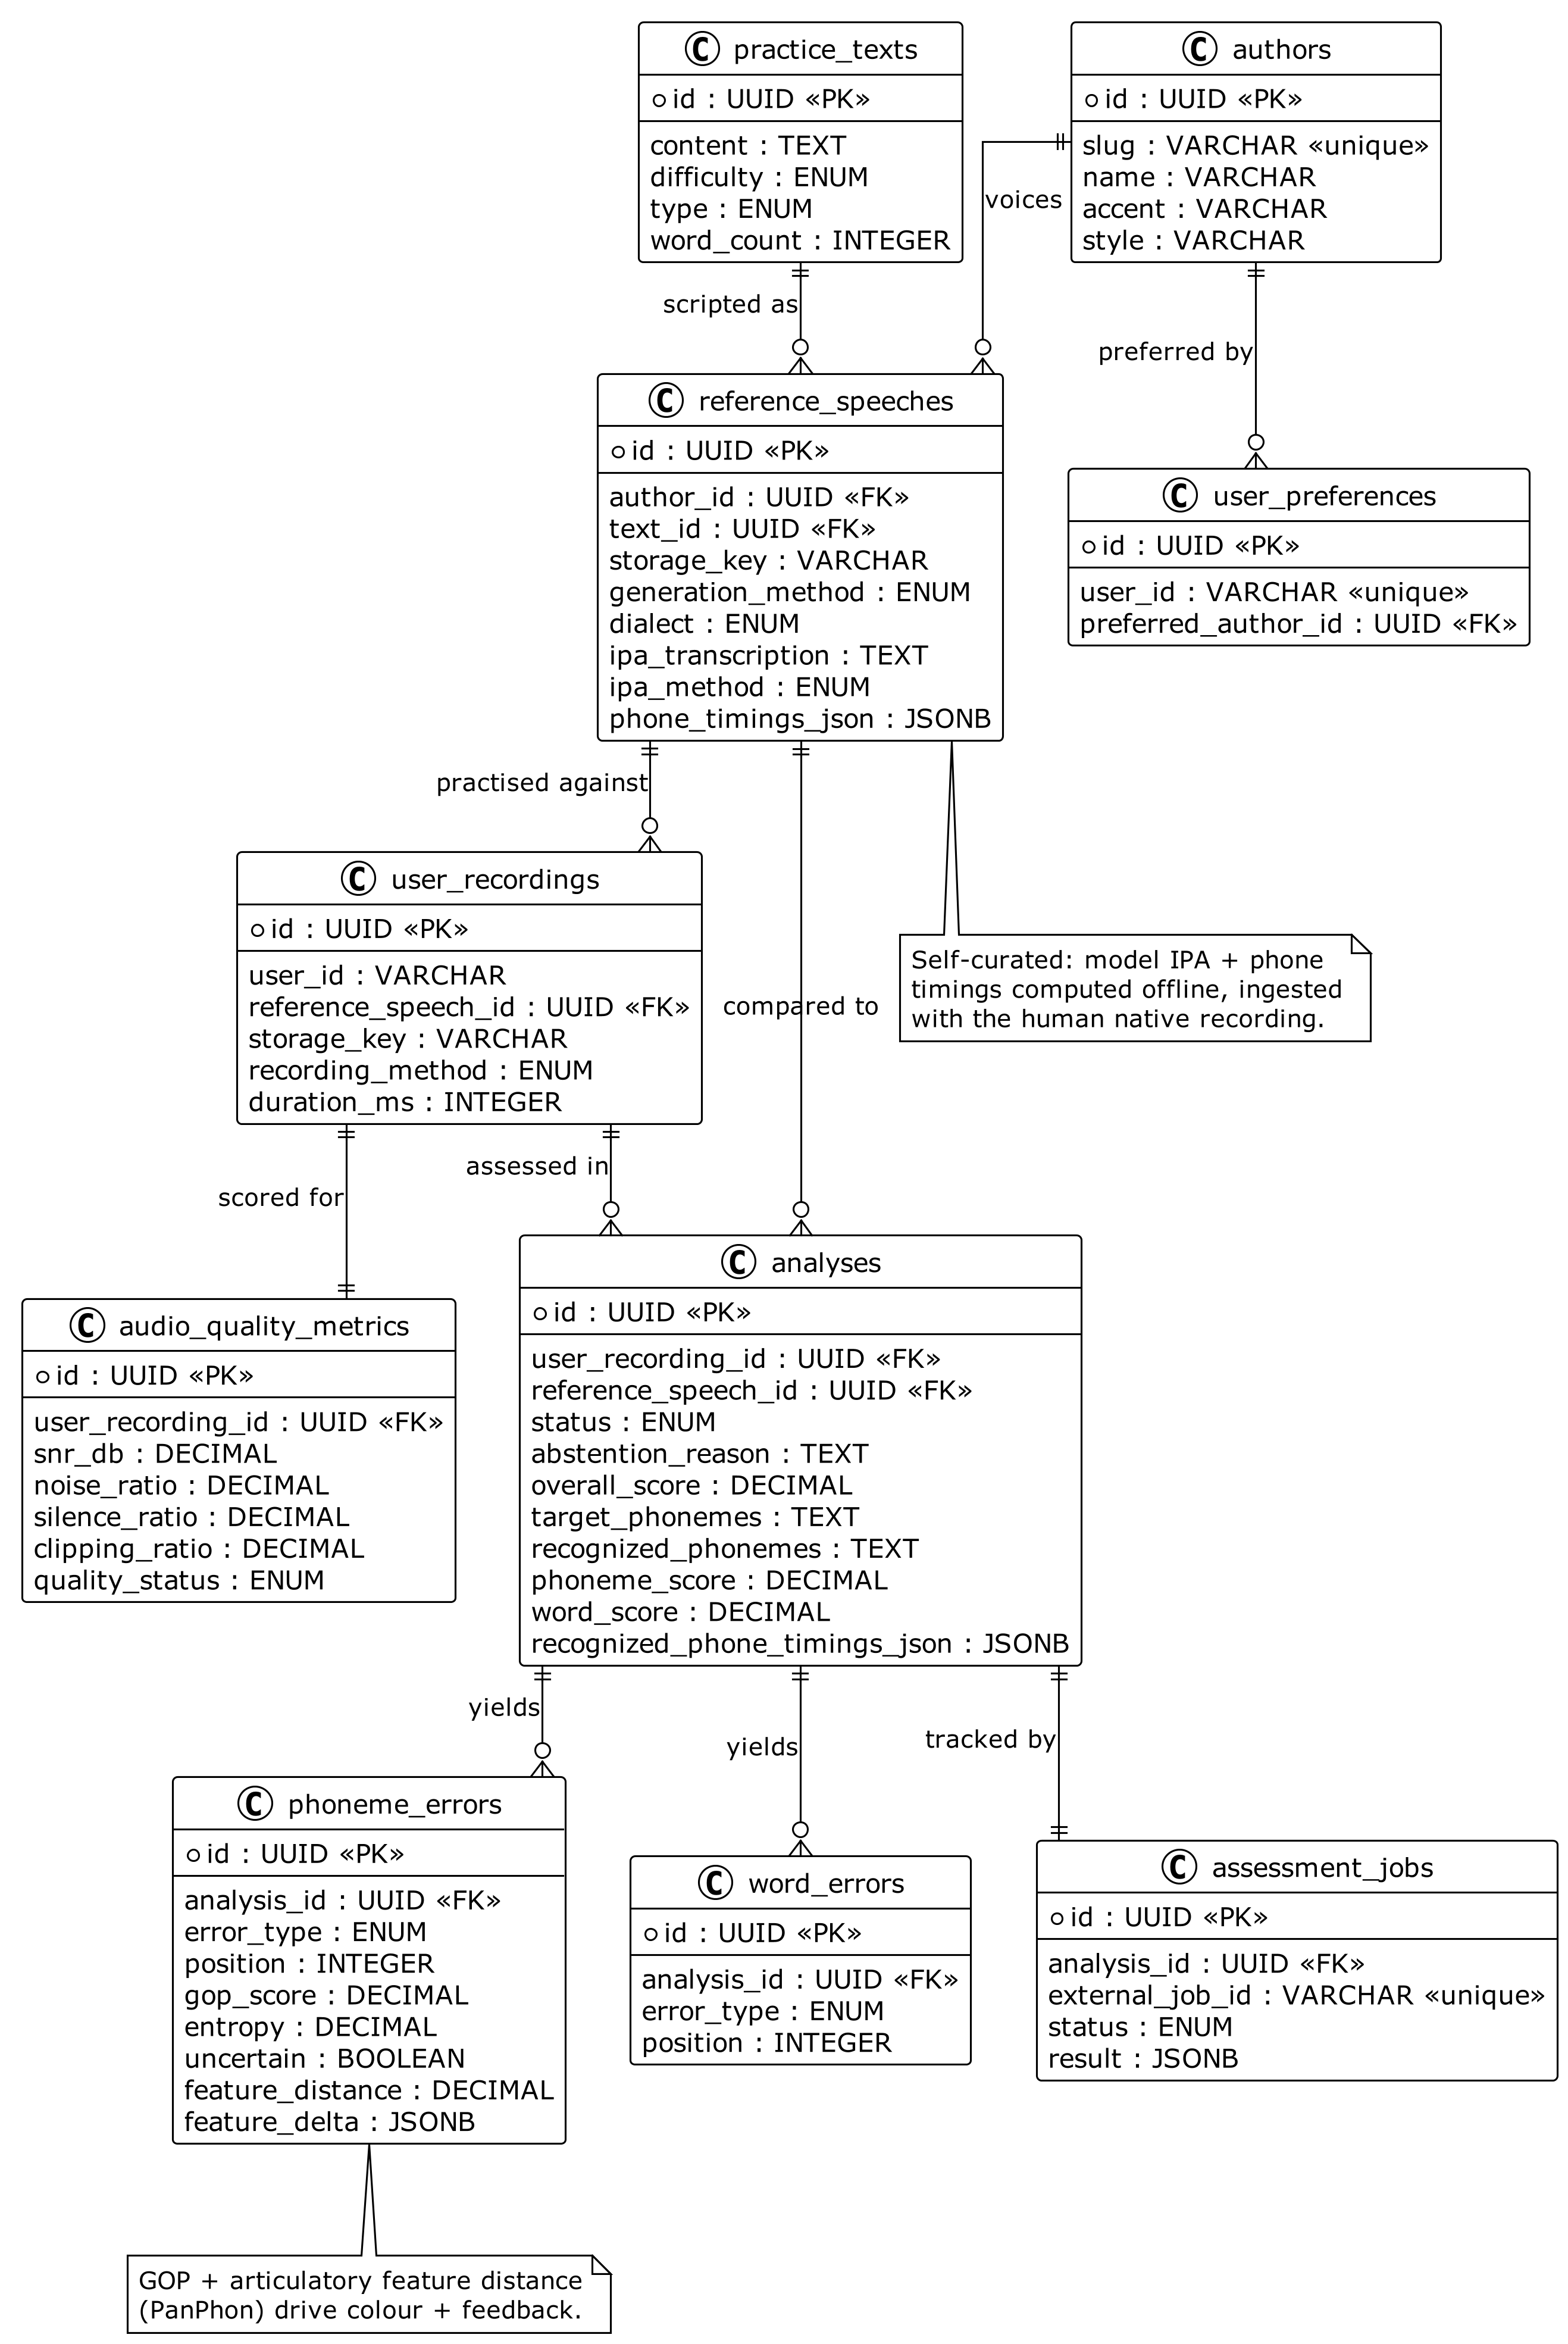
\includegraphics[width=\textwidth]{images/er-diagram.png}
\caption{Entity-Relationship Diagram for Nounce (Planned Schema)}
\label{fig:er-diagram}
\end{figure}

\section{Information Flow}

\subsection{Pronunciation Assessment Workflow}

\begin{figure}[H]
\centering
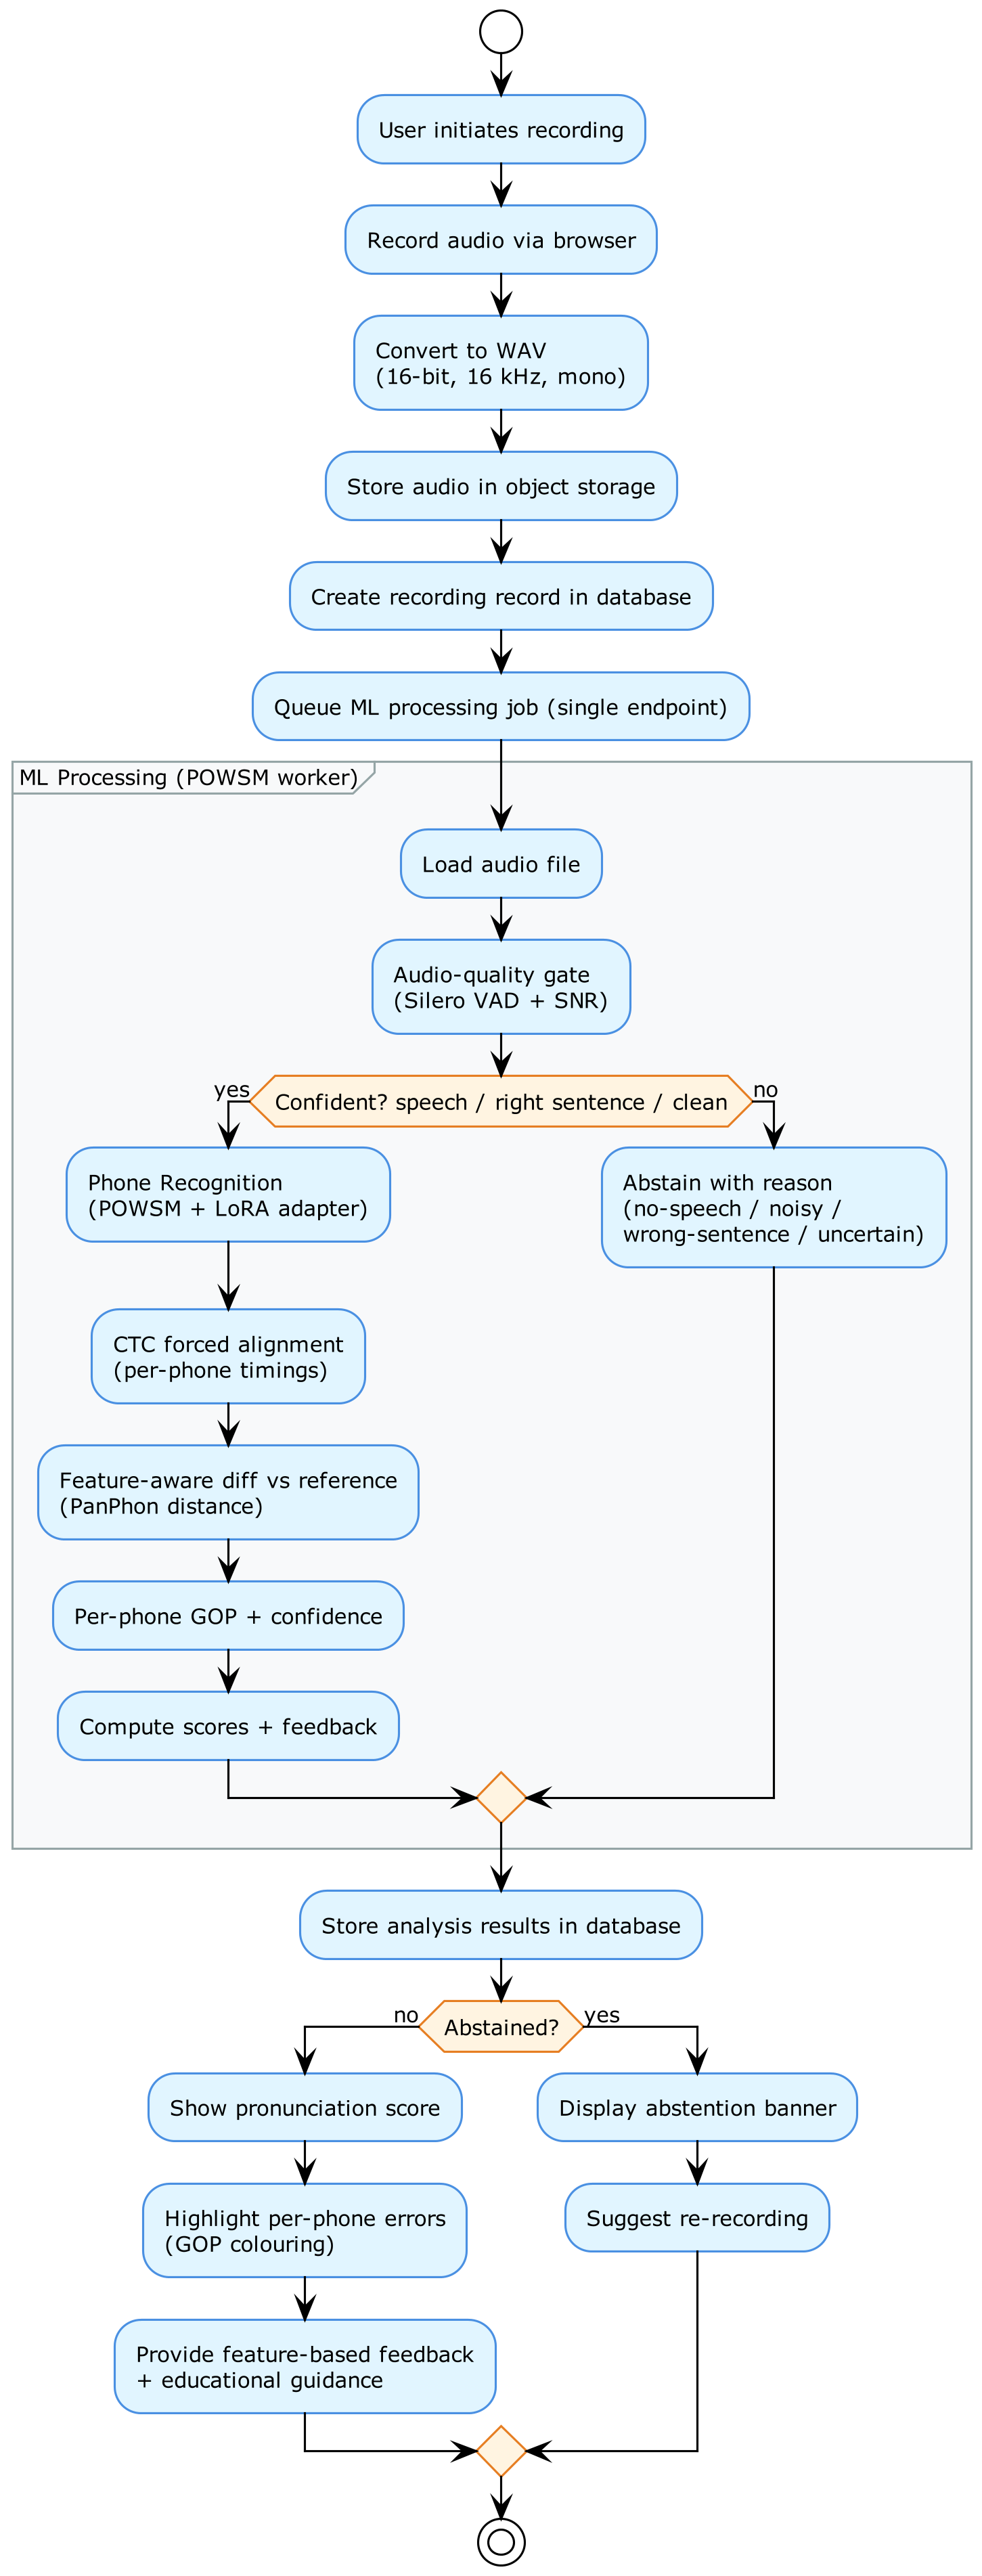
\includegraphics[height=1\textwidth]{images/activity-diagram.png}
\caption{Activity Diagram: Pronunciation Assessment Workflow}
\label{fig:activity-diagram}
\end{figure}

\section{System Design}

\subsection{System Architecture Diagram}

\begin{figure}[H]
\centering
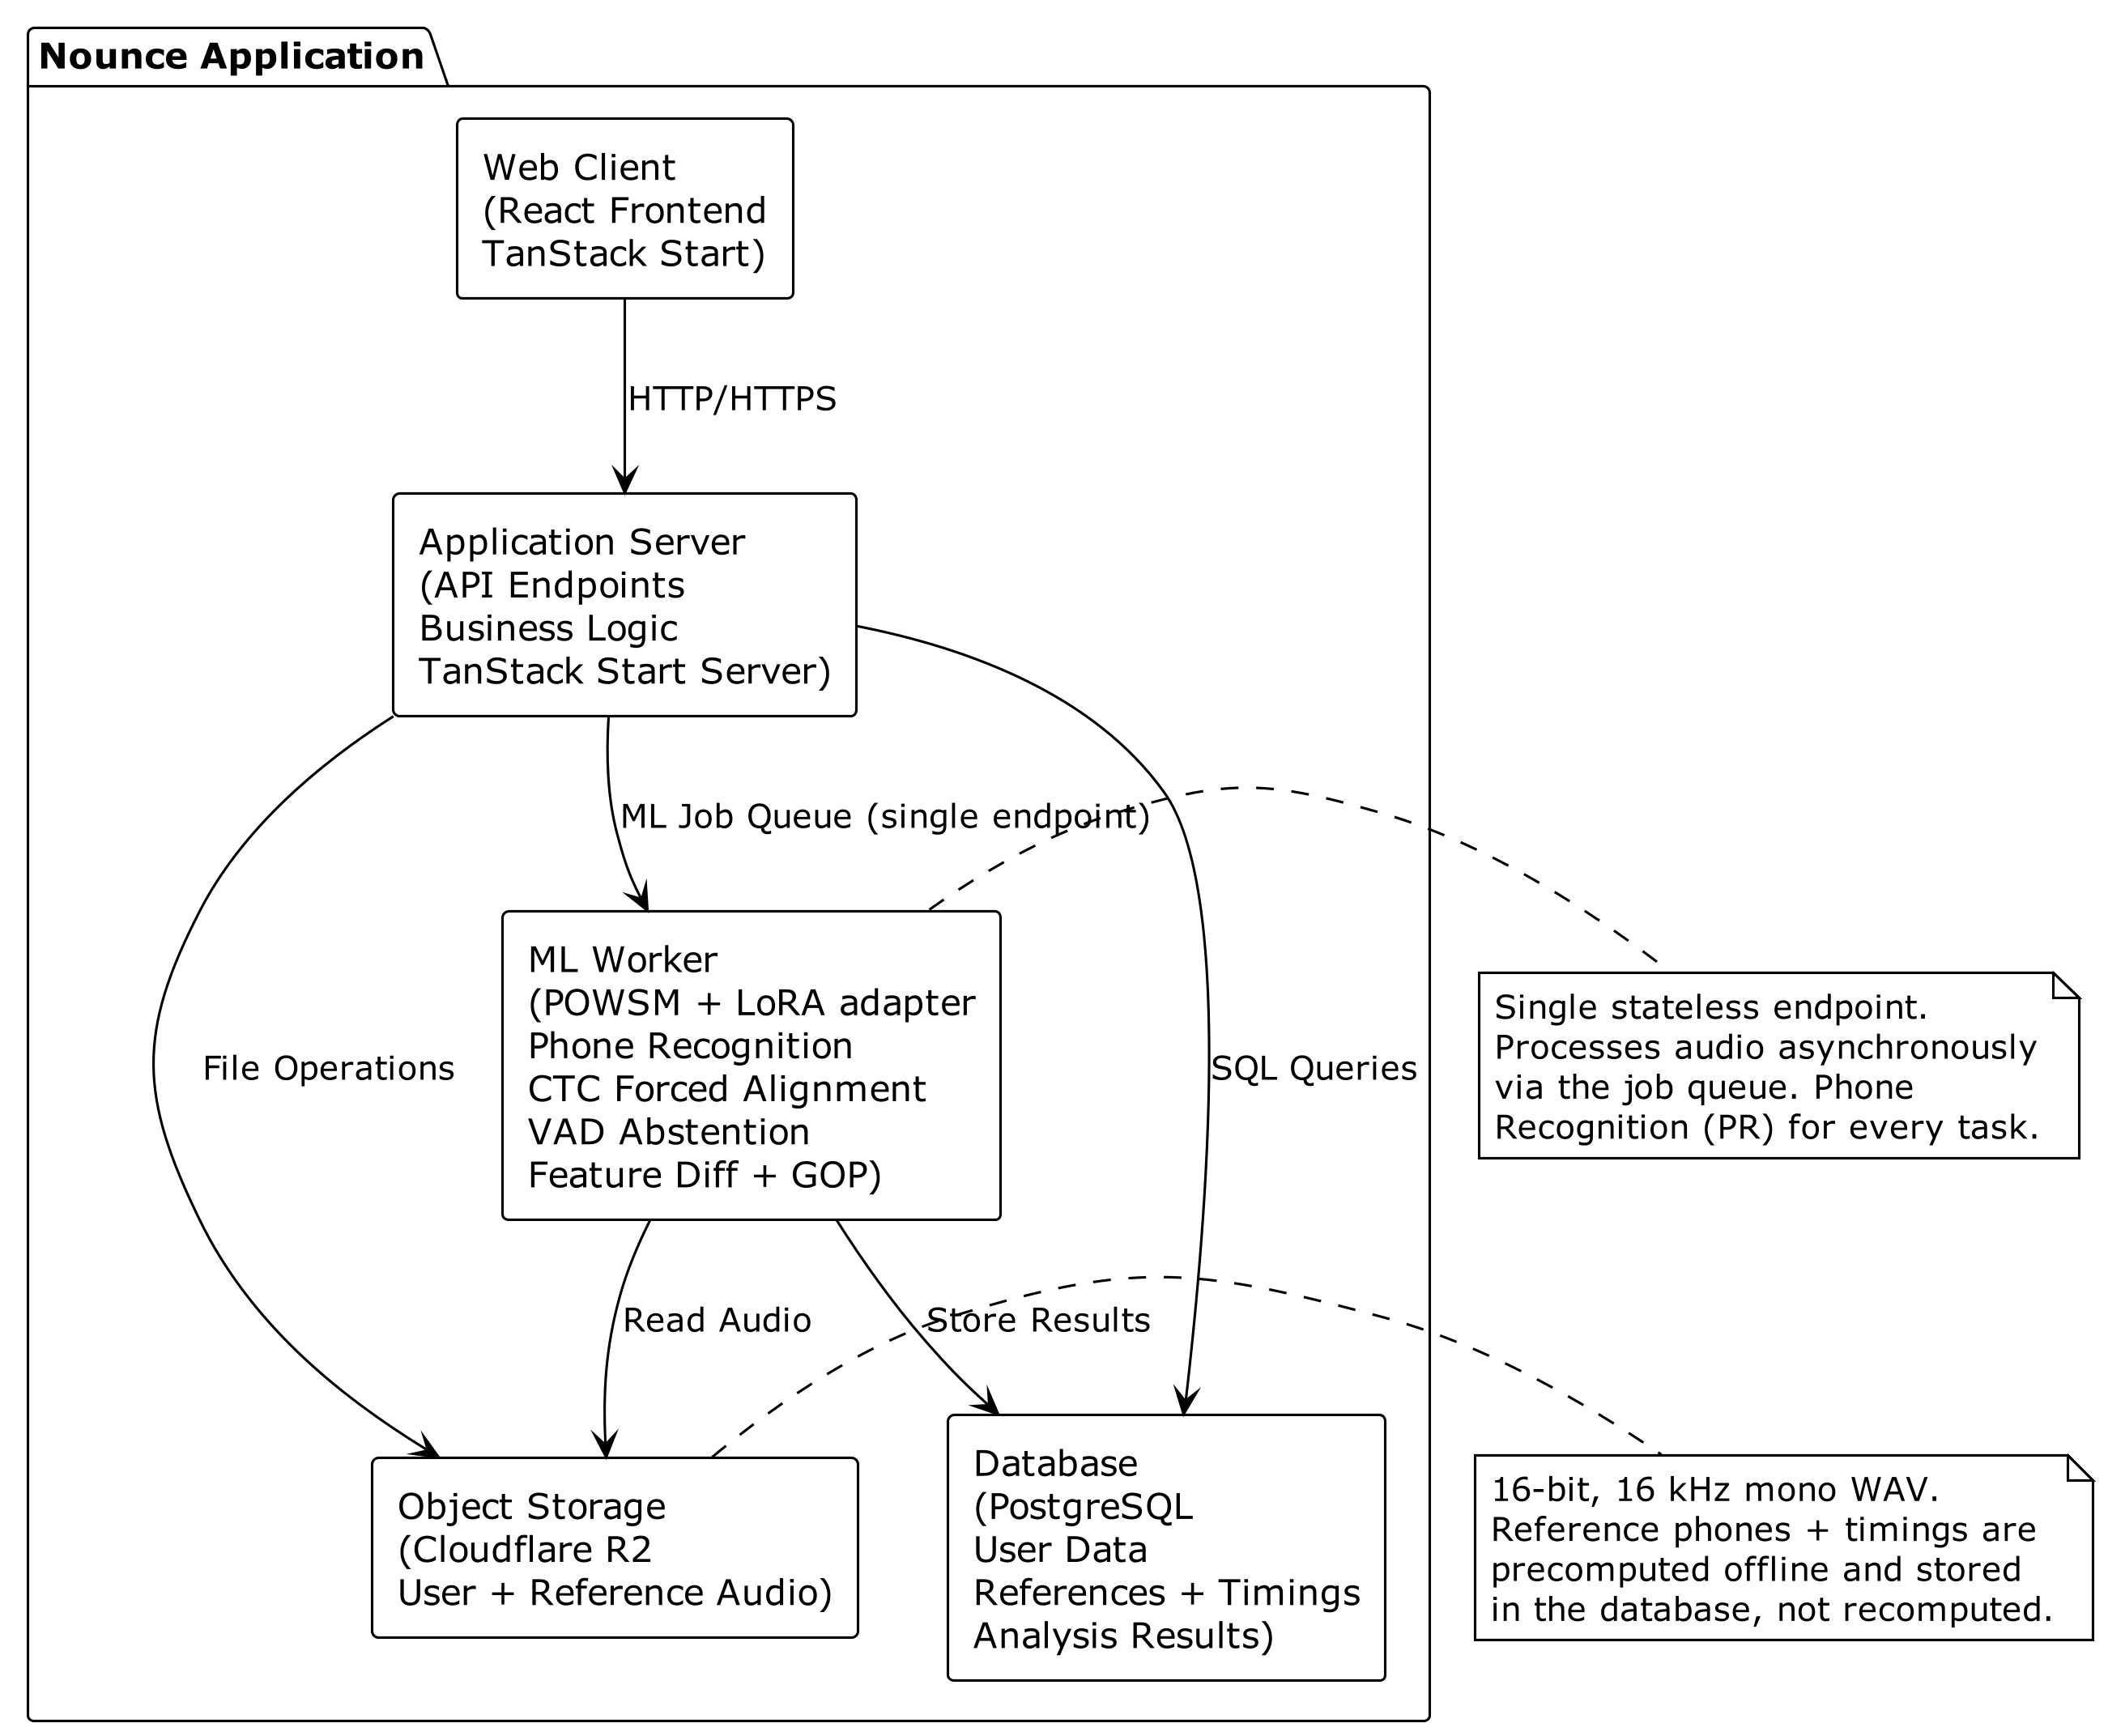
\includegraphics[width=\textwidth]{images/system-design.png}
\caption{System Architecture Diagram for Nounce}
\label{fig:system-design}
\end{figure}

\subsection{Deployment Architecture Diagram}

\begin{figure}[H]
\centering
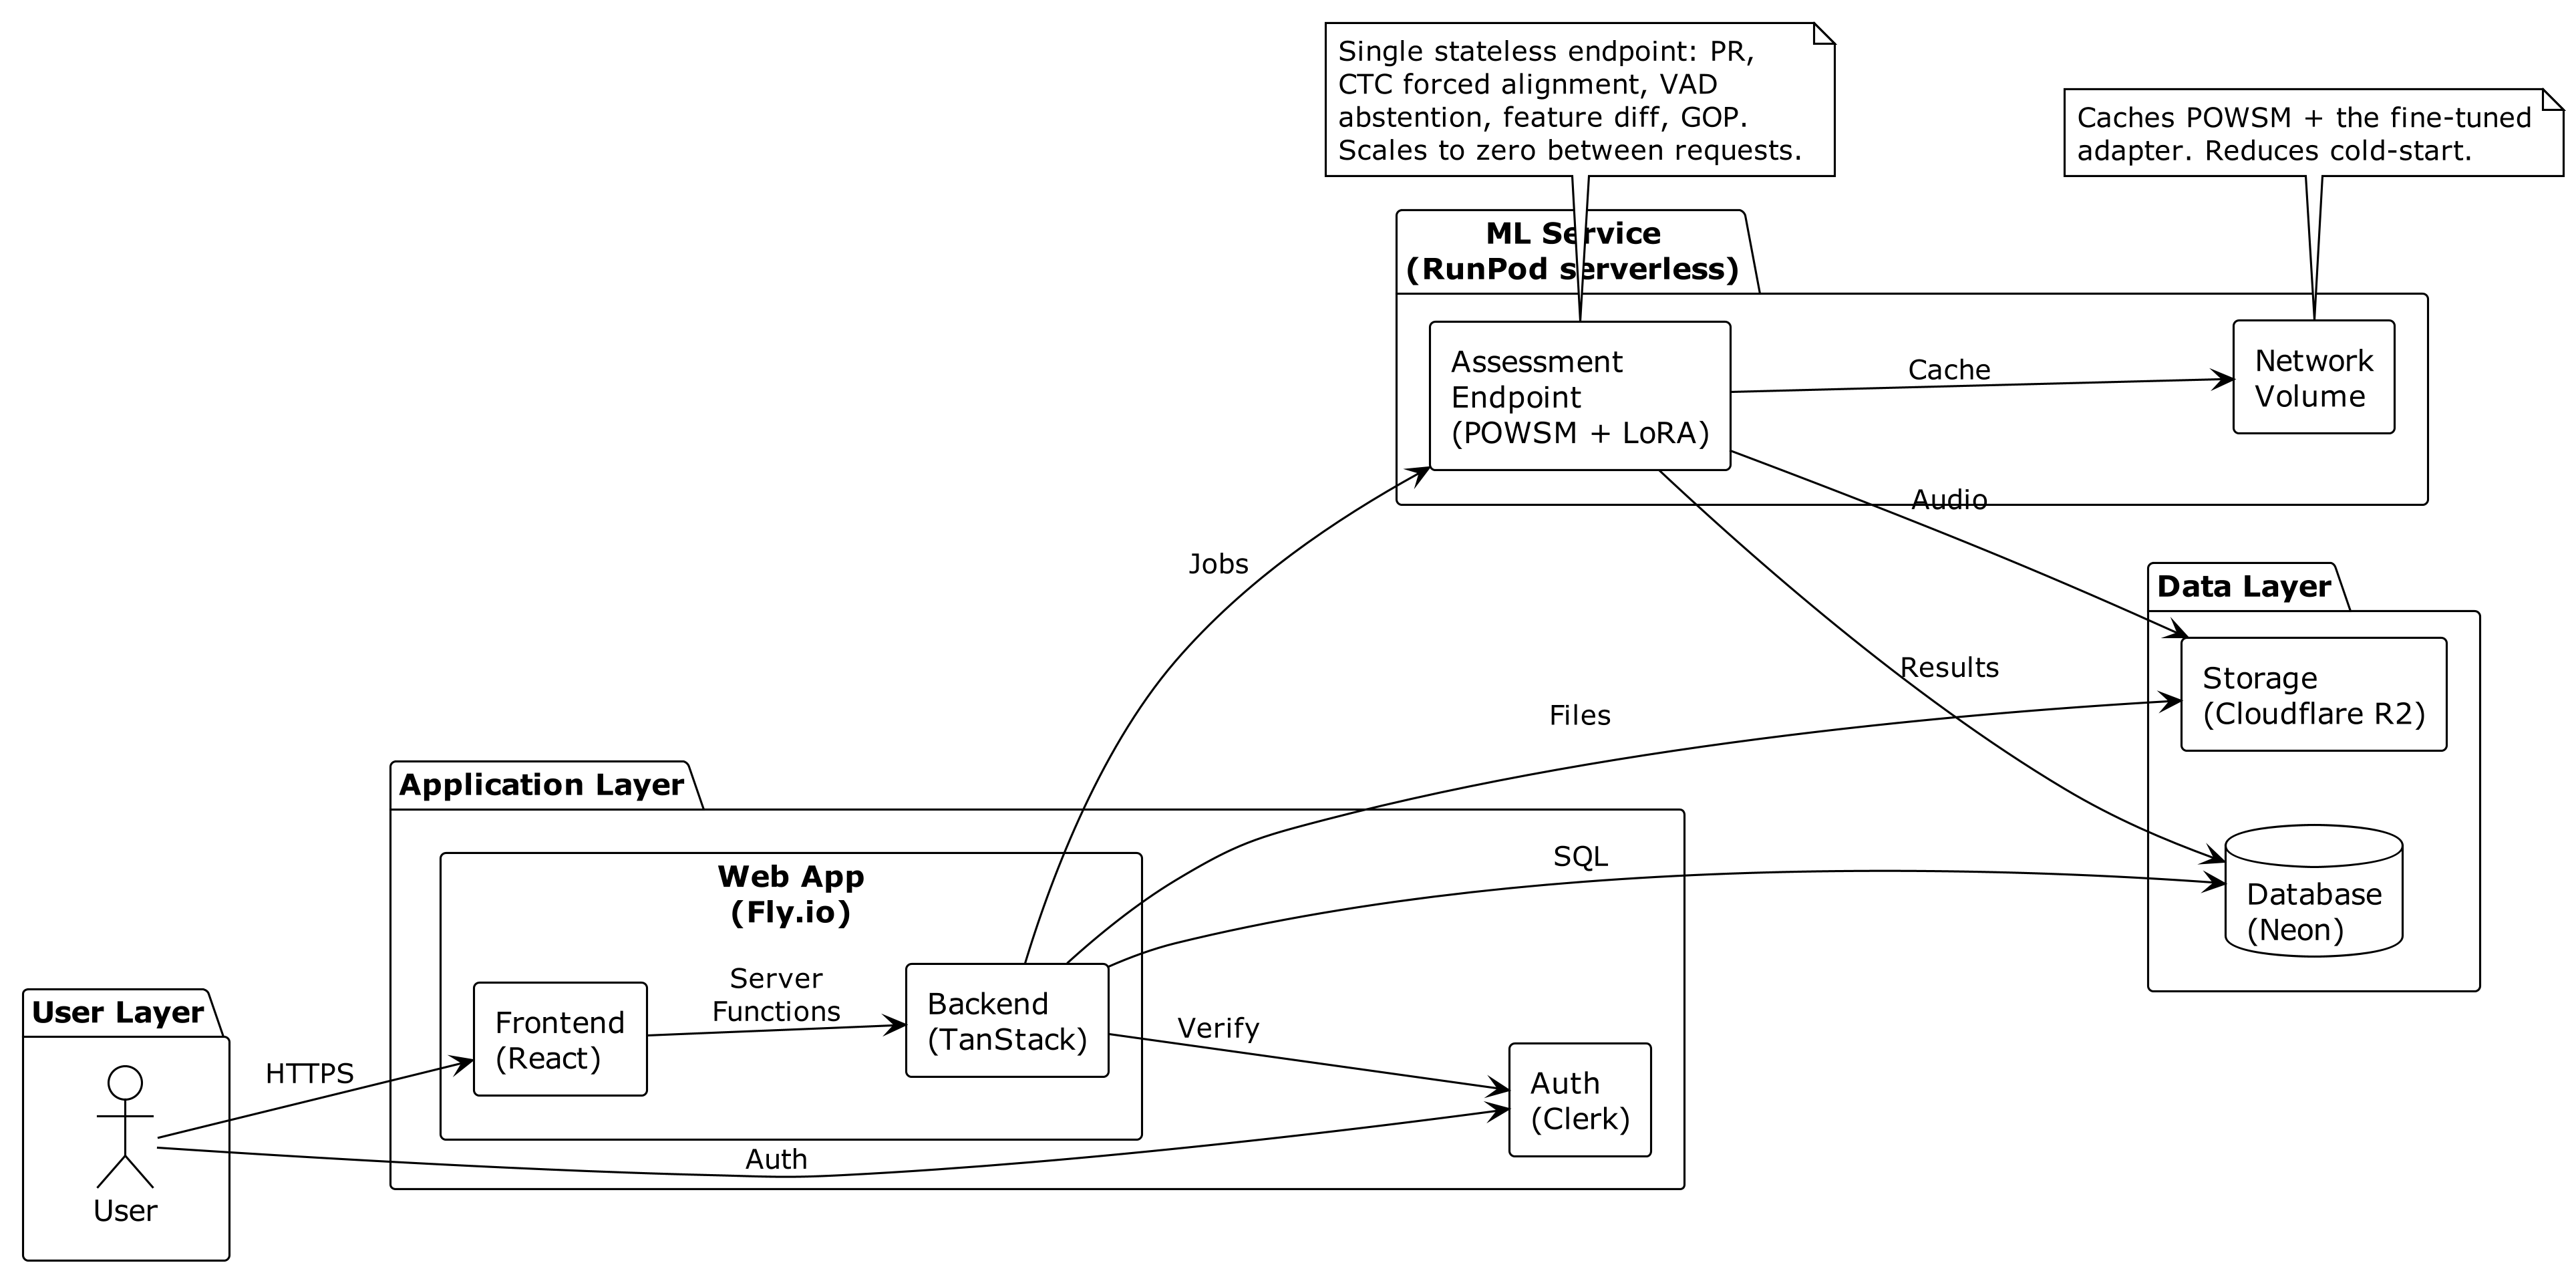
\includegraphics[width=0.95\textwidth,angle=0]{images/deployment-architecture.png}
\caption{Production Deployment Architecture}
\label{fig:deployment-architecture}
\end{figure}

\subsection{RunPod Simulator Architecture Diagram}

\begin{figure}[H]
\centering
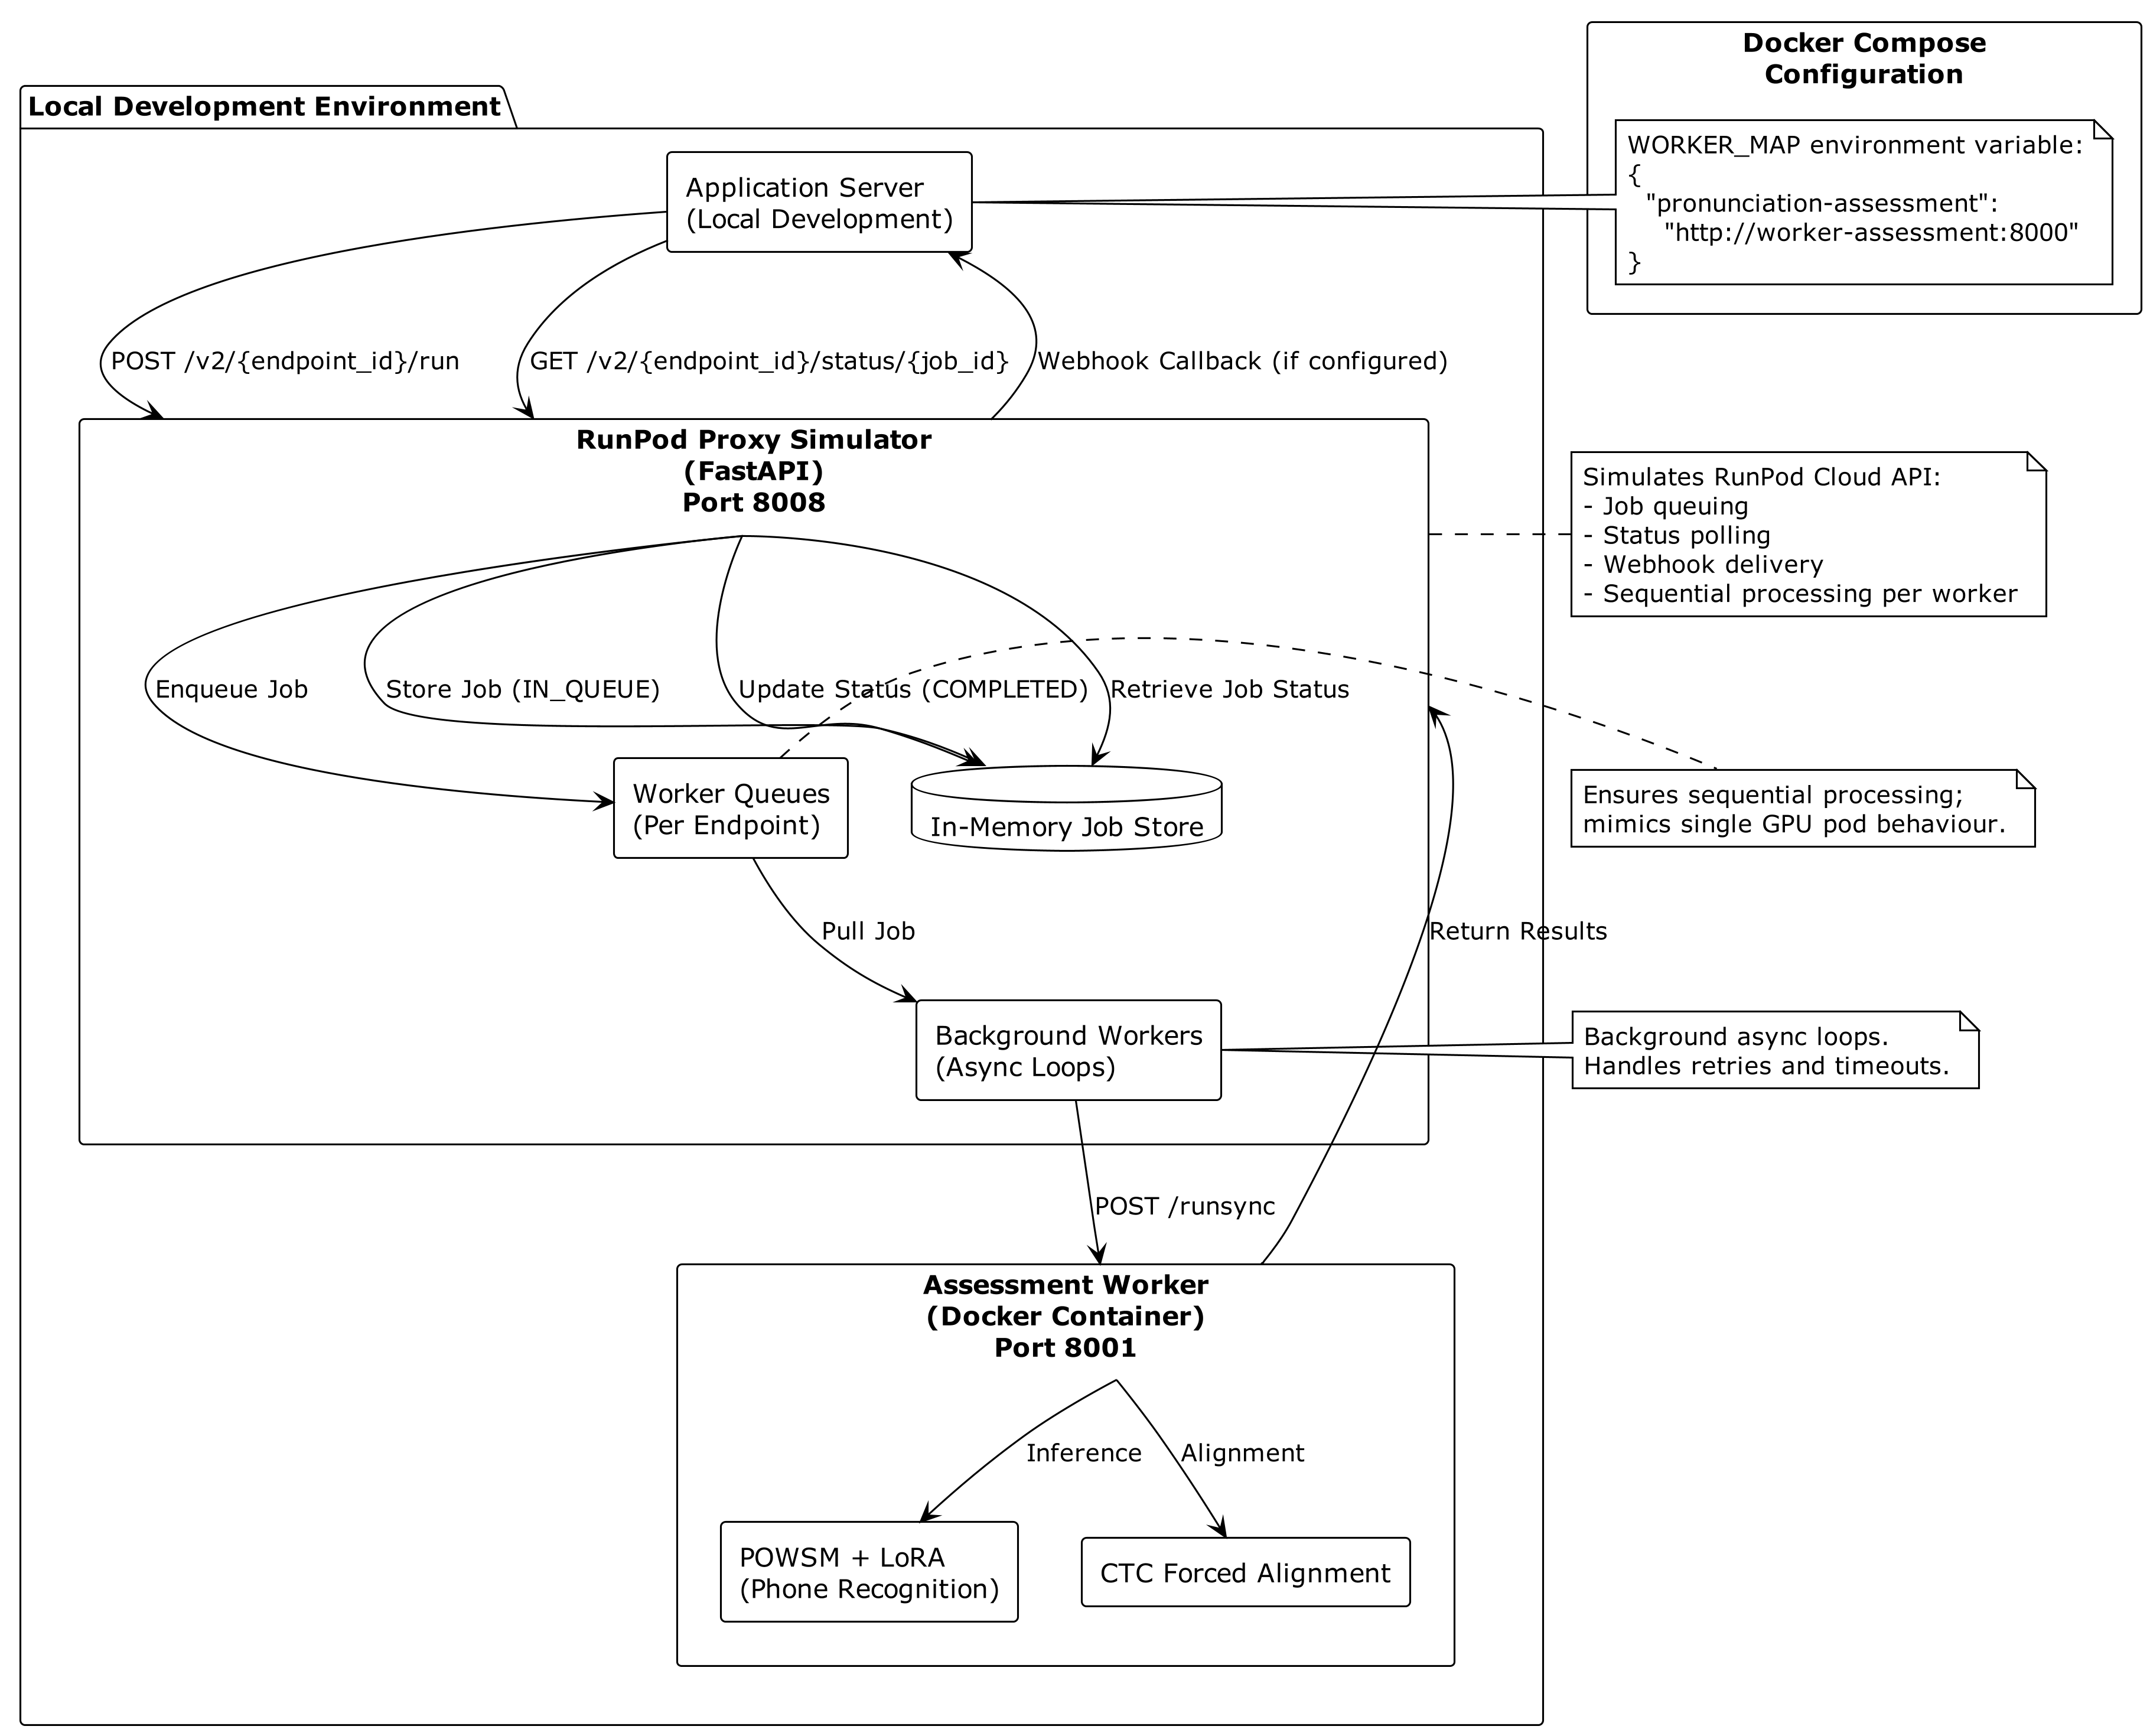
\includegraphics[width=\textwidth]{images/runpod-simulator.png}
\caption{Local RunPod Serverless Simulator Architecture}
\label{fig:runpod-simulator}
\end{figure}

\section{User Interface Design}

\subsection{Application Logo}

\begin{figure}[H]
\centering

\includegraphics[width=0.8\textwidth]{images/frame.png}
\caption{Nounce Application Logo}
\label{fig:nounce-logo}
\end{figure}

\subsection{User Interface Screenshots}

The Nounce application provides a modern, intuitive user interface built with Shadcn UI and ElevenLabs UI components. The following screenshots demonstrate key features and workflows of the application. All screenshots are captured in dark mode.

\subsubsection{Home Page}

\begin{figure}[H]
\centering
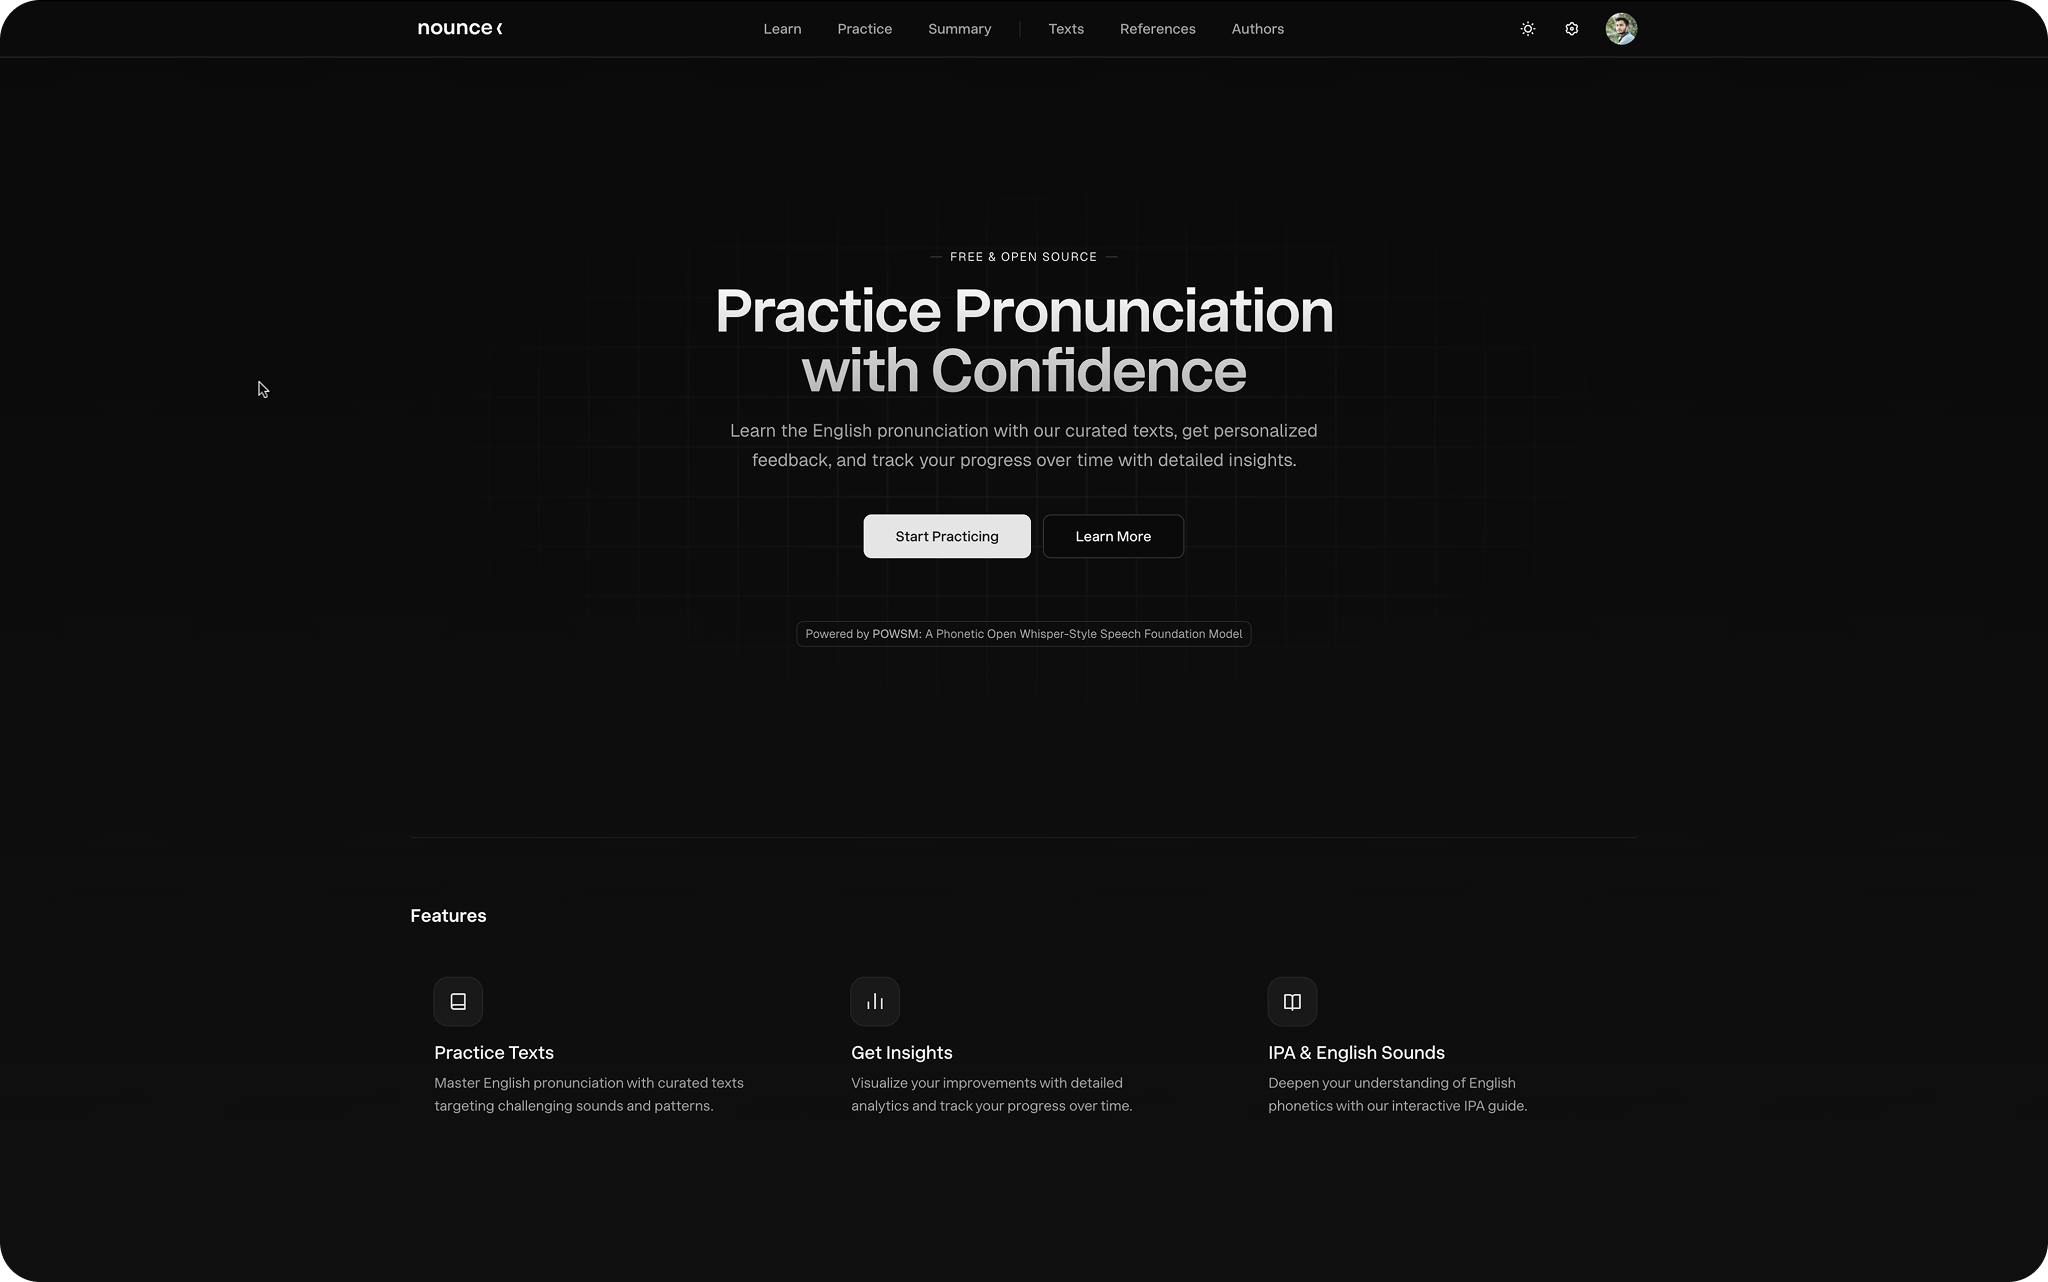
\includegraphics[width=\textwidth]{images/screen/nounce-ss-home.png}
\caption{Home Page - Main landing page with feature overview and navigation}
\label{fig:ui-home}
\end{figure}

\subsubsection{Practice Text Selection}

\begin{figure}[H]
\centering
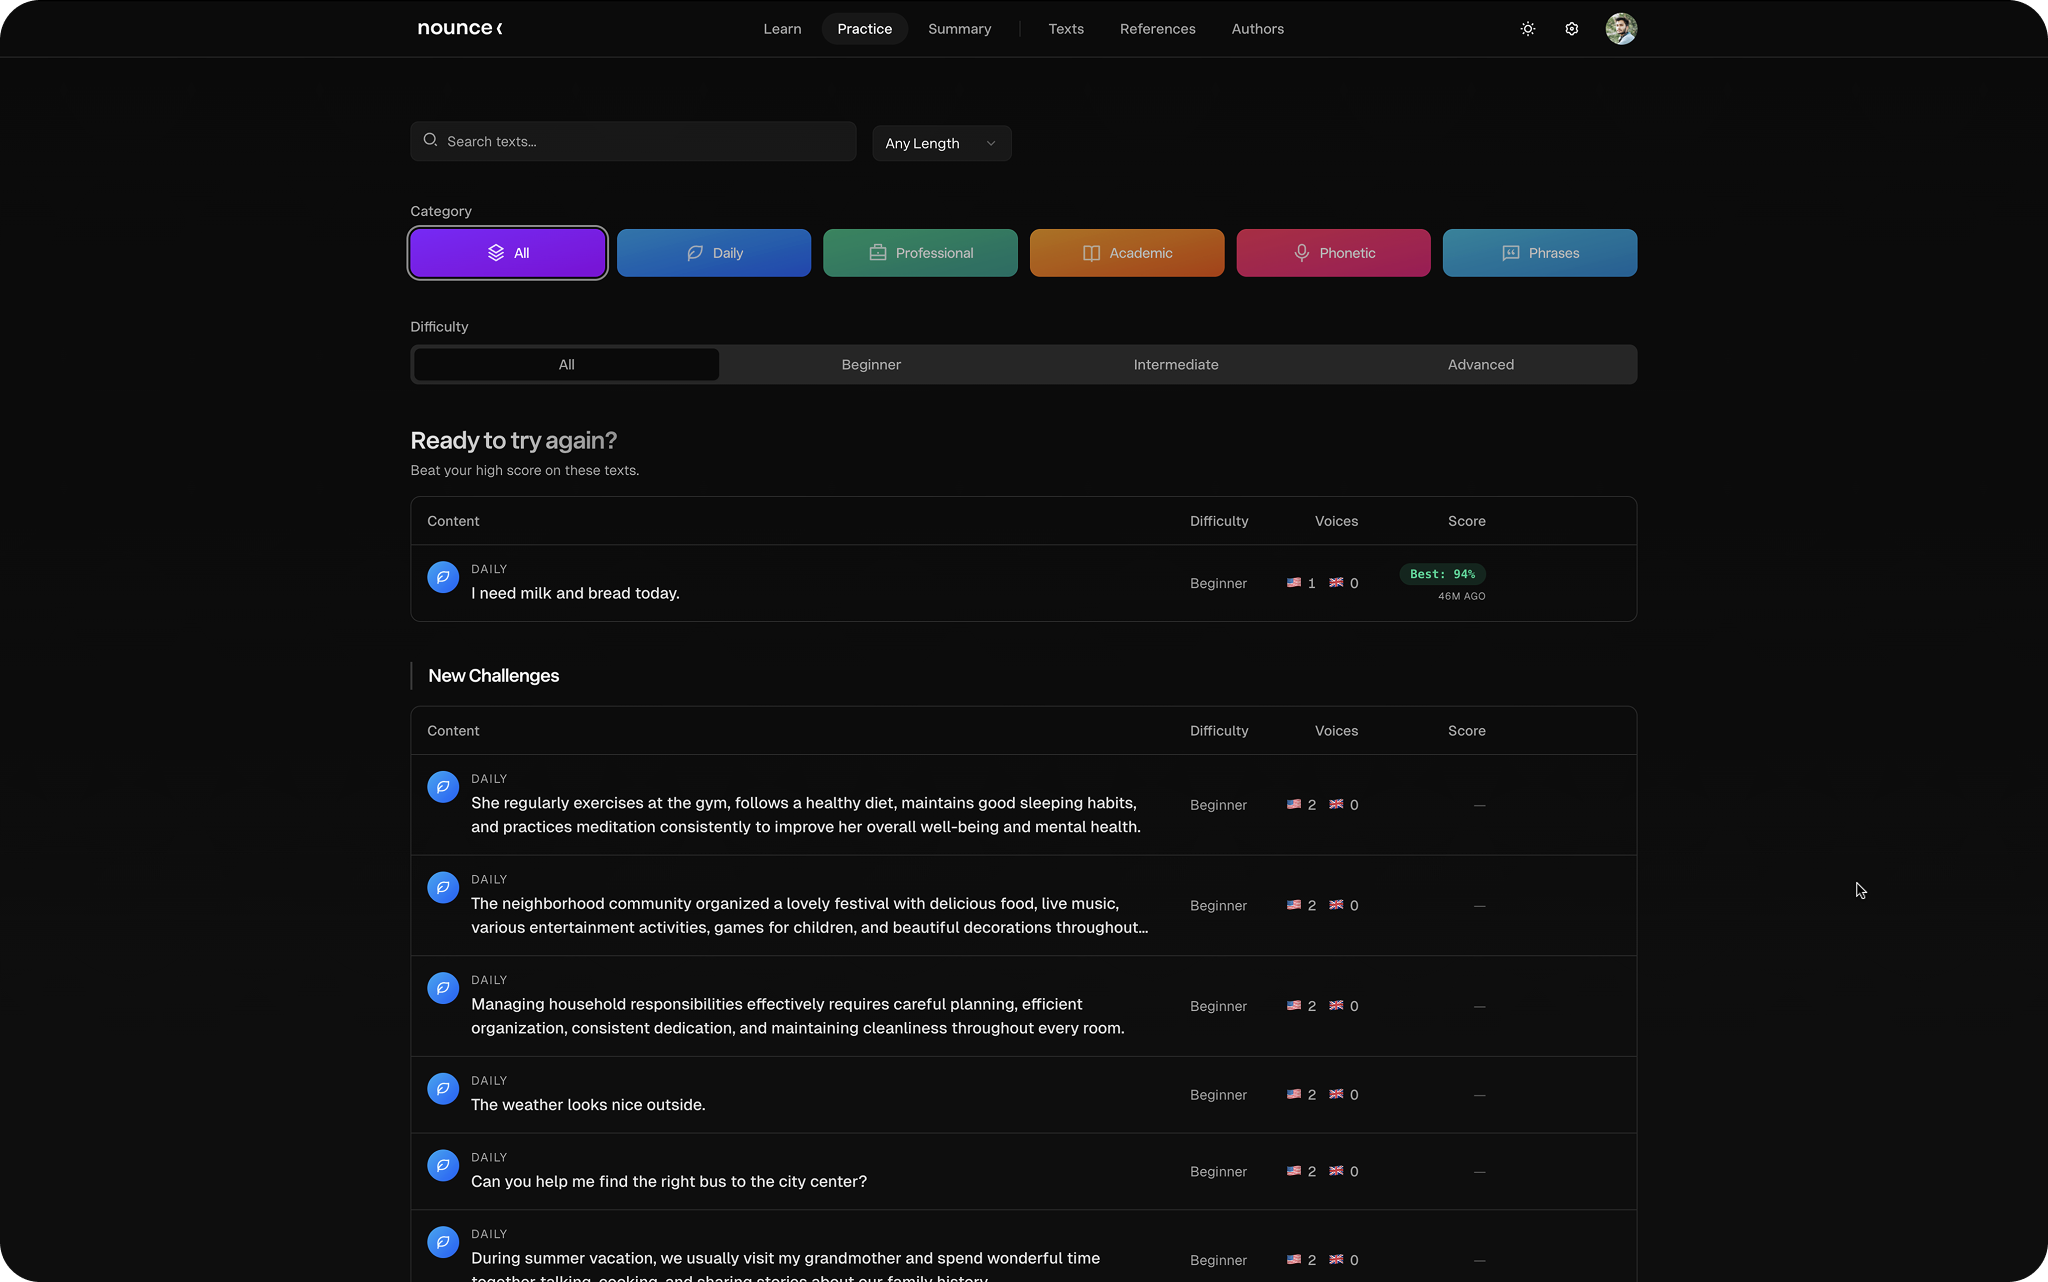
\includegraphics[width=\textwidth]{images/screen/nounce-ss-practice.png}
\caption{Practice Text Selection - Browse and filter practice texts by difficulty and category}
\label{fig:ui-practice-selection}
\end{figure}

\subsubsection{Recording Interface}

\begin{figure}[H]
\centering
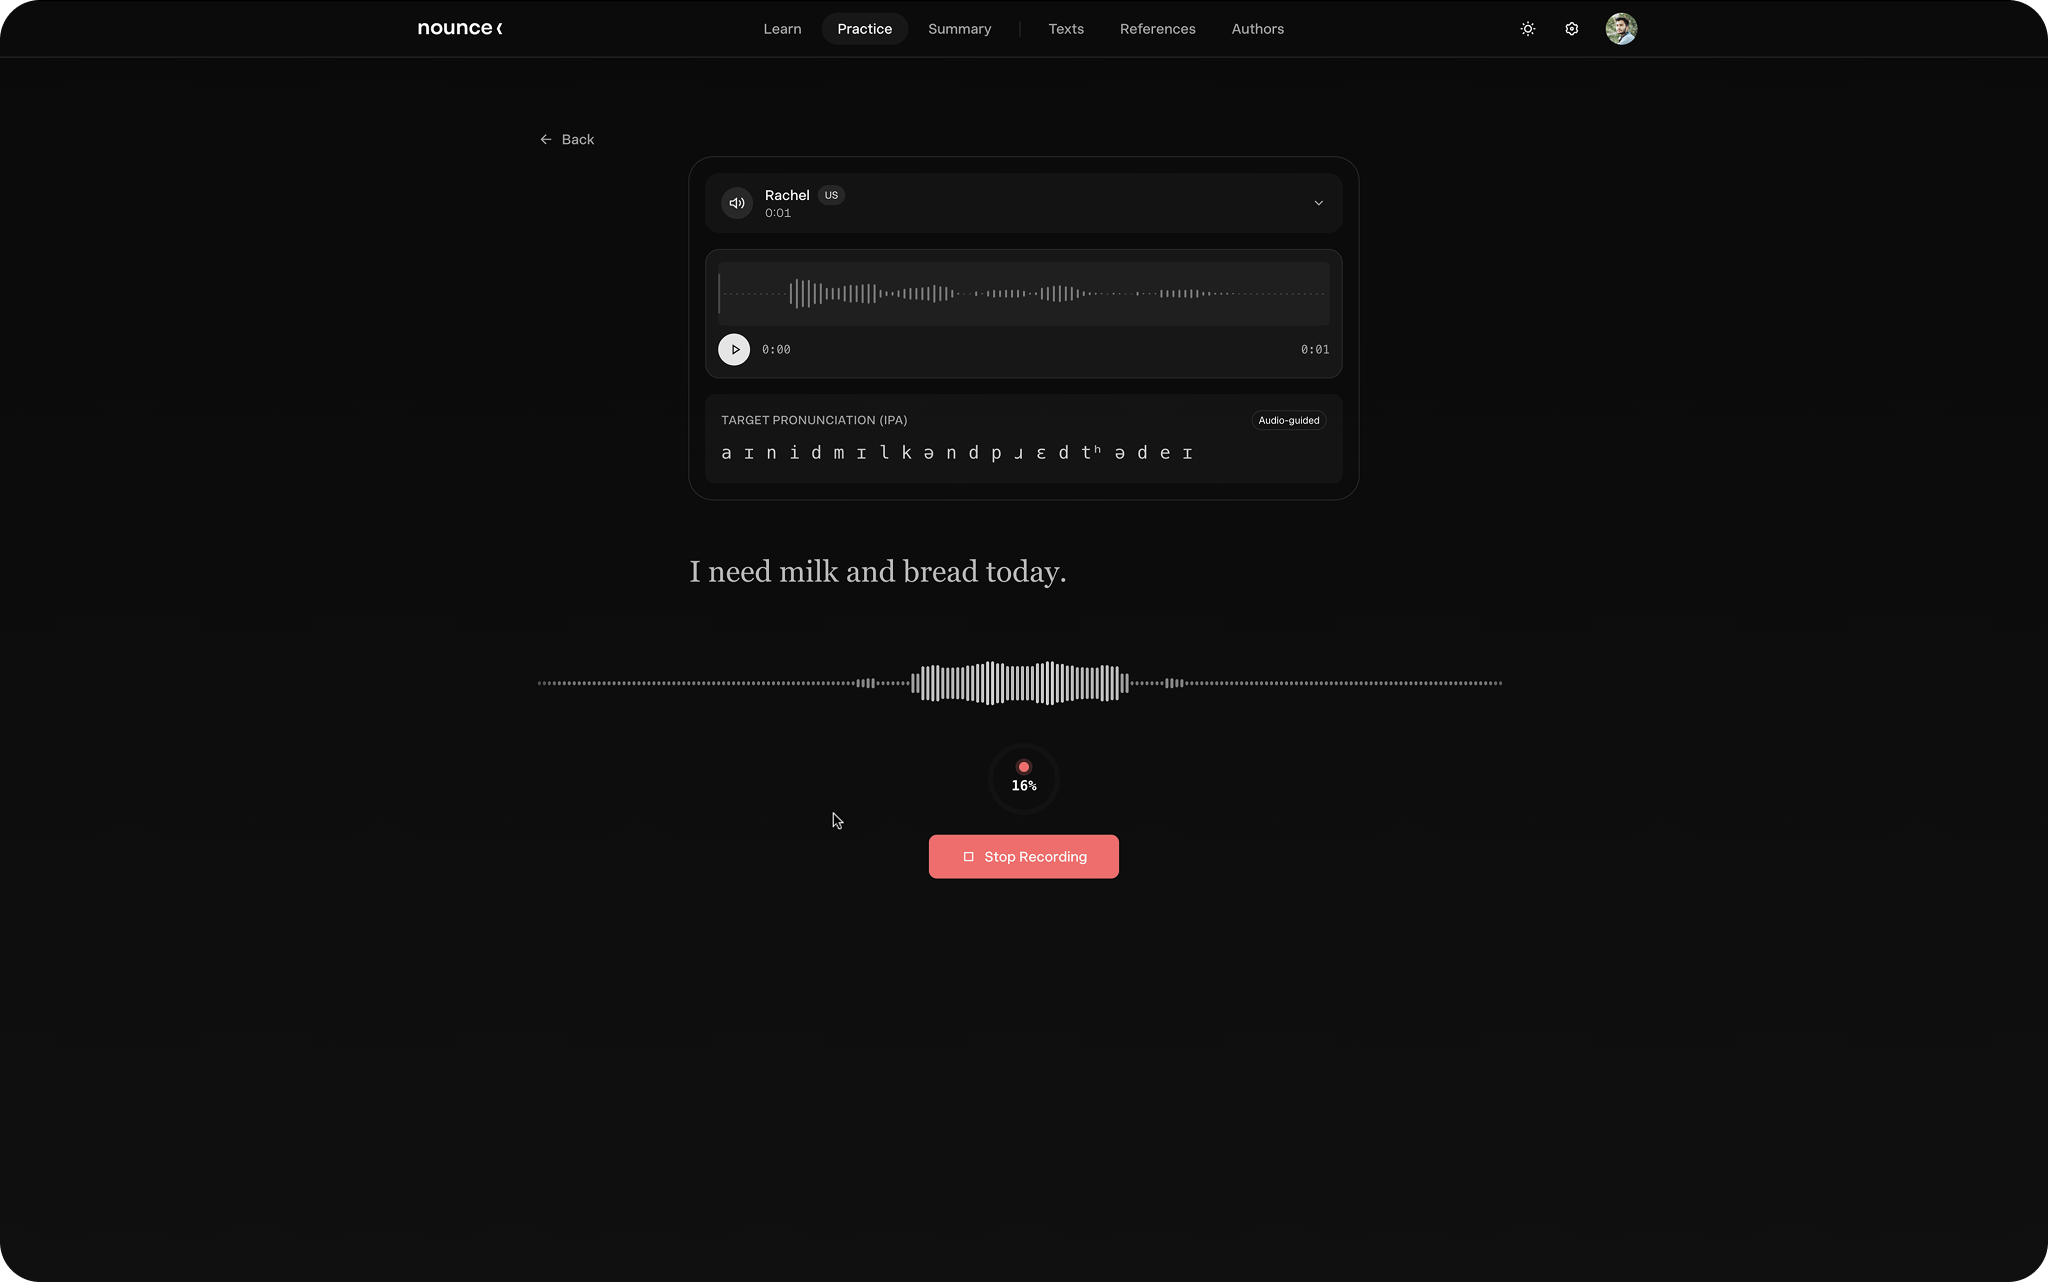
\includegraphics[width=\textwidth]{images/screen/nounce-ss-recording.png}
\caption{Recording Interface - Browser-based audio recording with real-time waveform visualization (dark mode)}
\label{fig:ui-recording}
\end{figure}

\subsubsection{Analysis Results}

\begin{figure}[H]
\centering
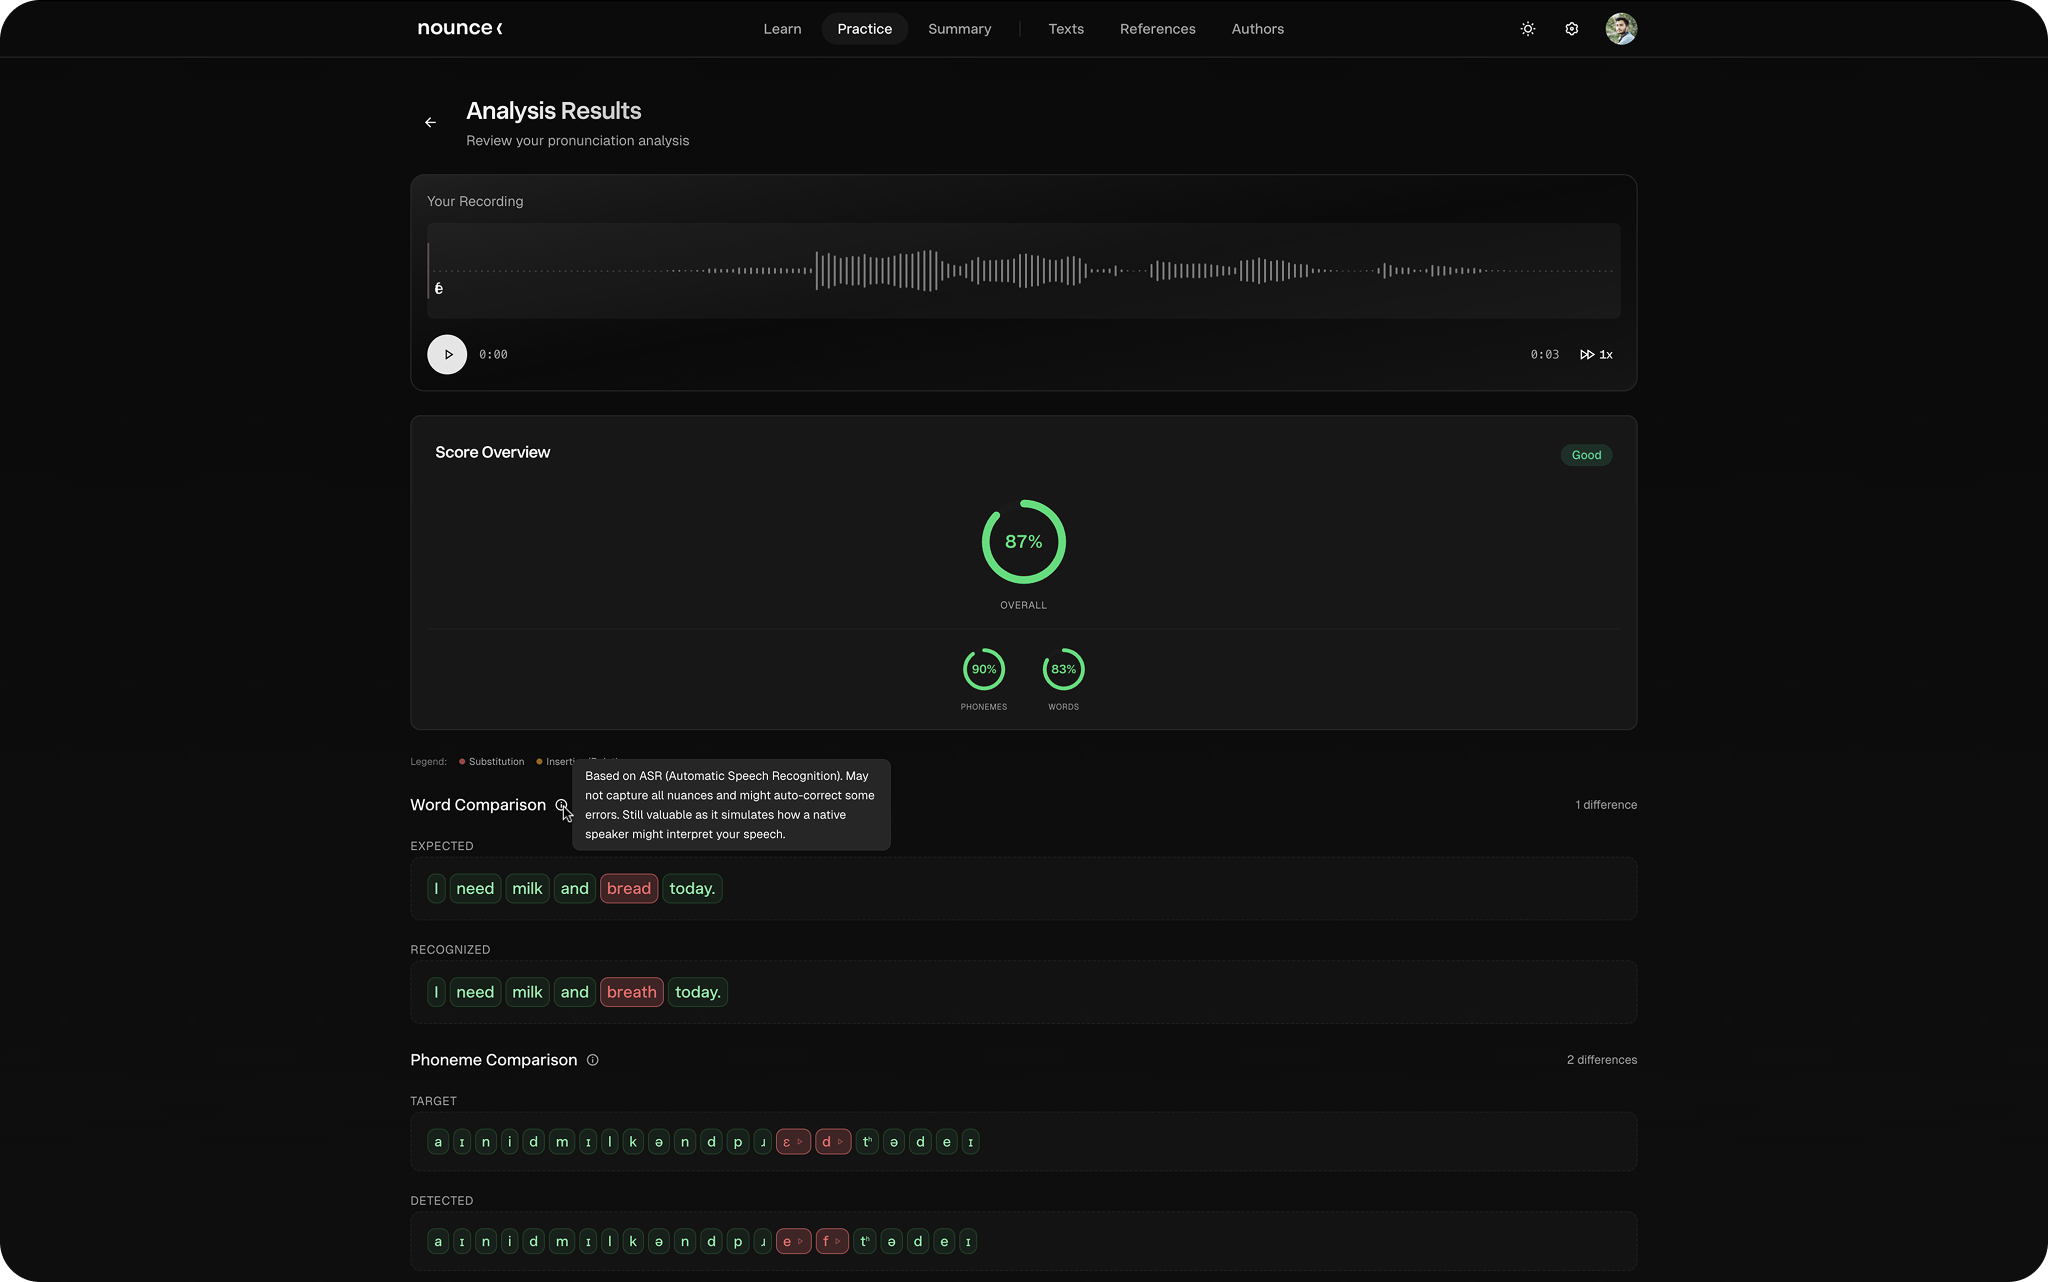
\includegraphics[width=\textwidth]{images/screen/nounce-ss-analysis.png}
\caption{Analysis Results - Detailed pronunciation feedback with phoneme and word-level error visualization}
\label{fig:ui-analysis}
\end{figure}

\subsubsection{Progress Dashboard}

\begin{figure}[H]
\centering
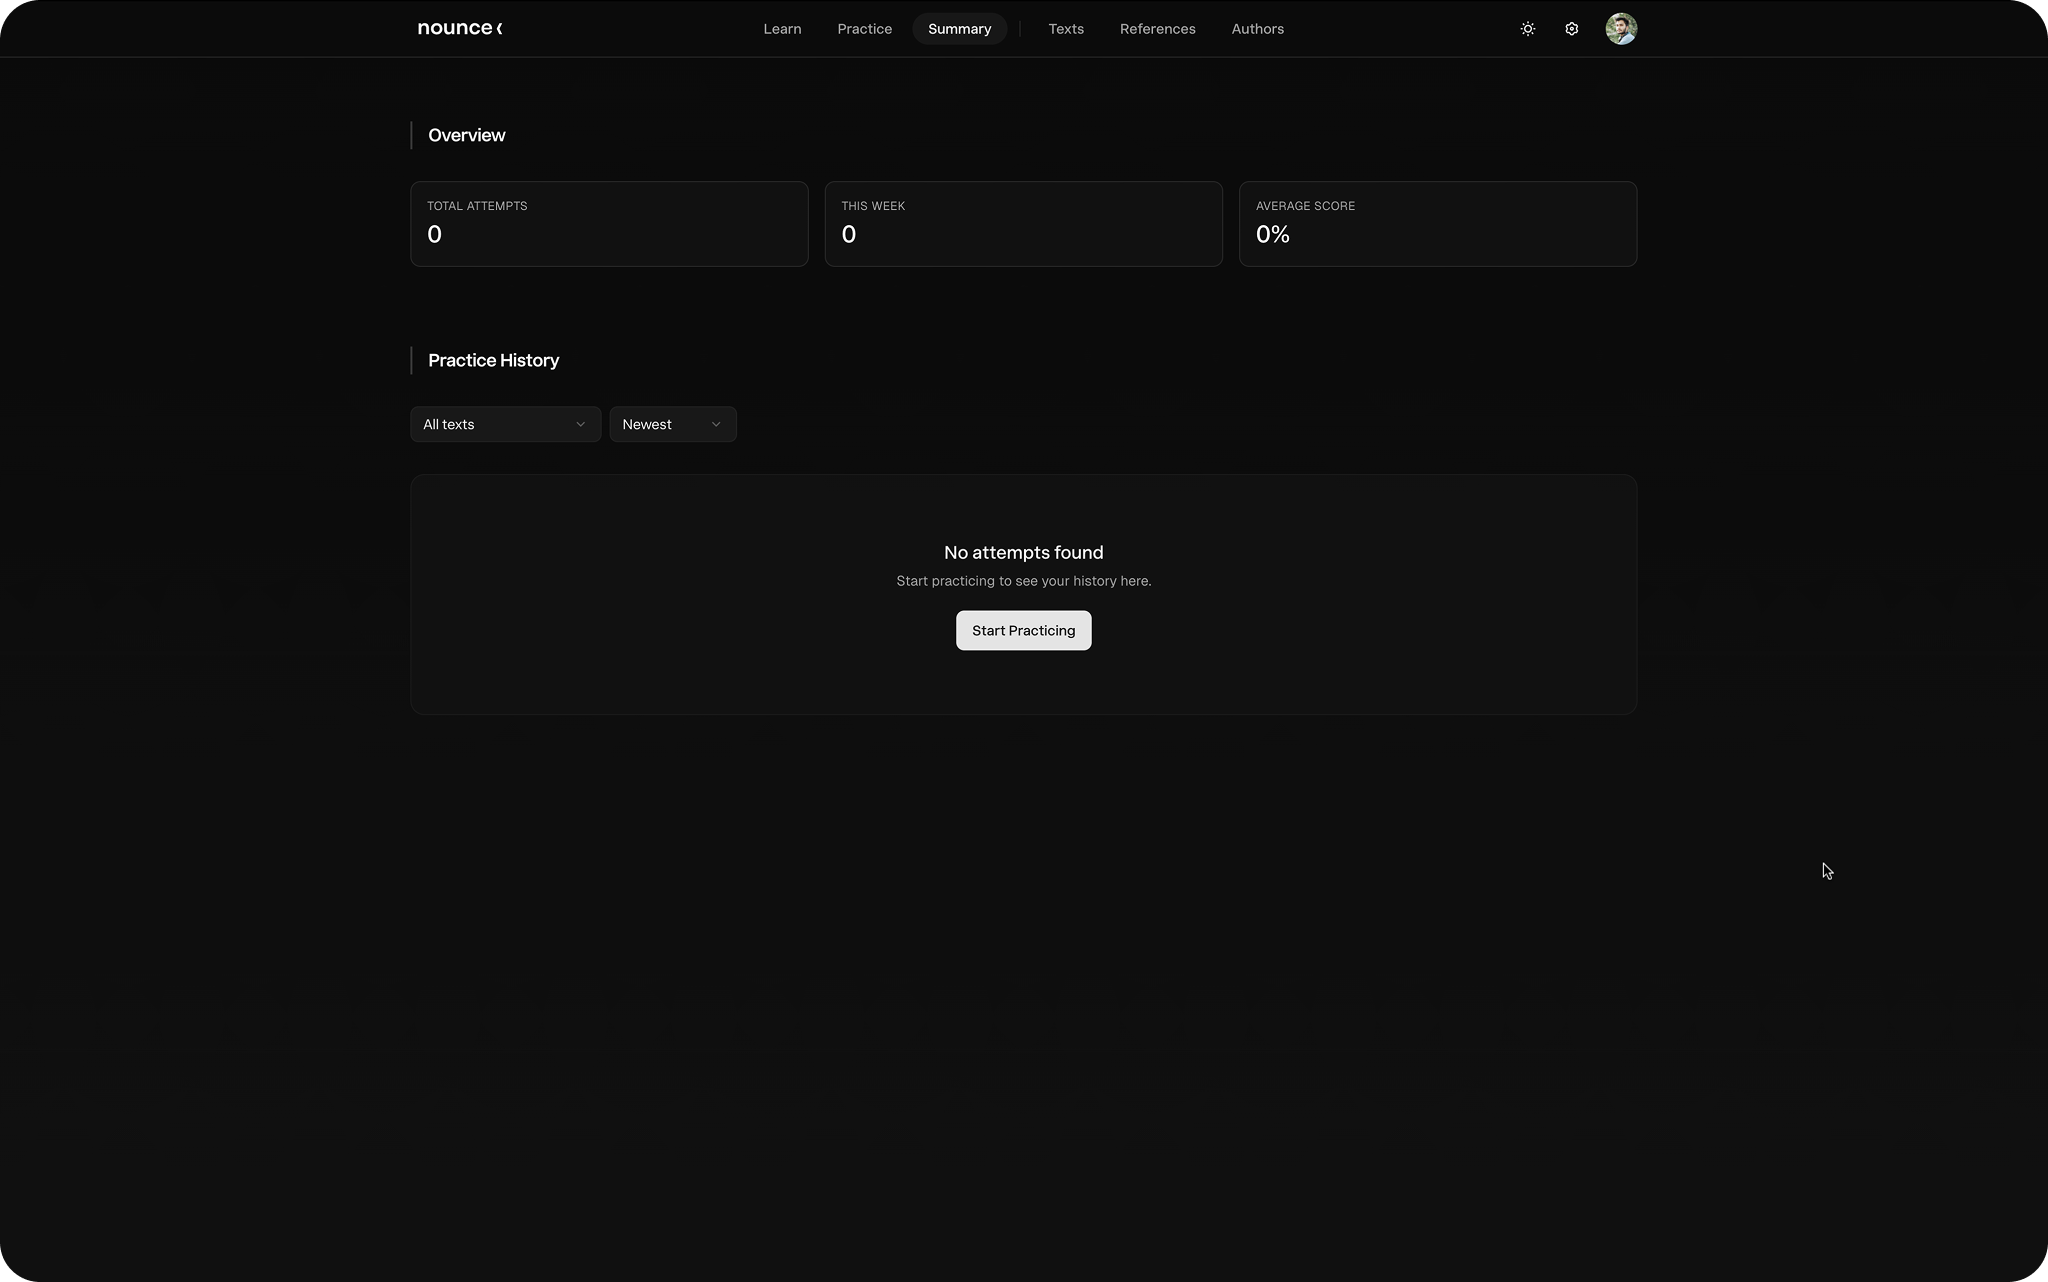
\includegraphics[width=\textwidth]{images/screen/nounce-ss-summary.png}
\caption{Progress Dashboard - User statistics and error analysis over time}
\label{fig:ui-summary}
\end{figure}

\subsubsection{Educational Content}

\begin{figure}[H]
\centering
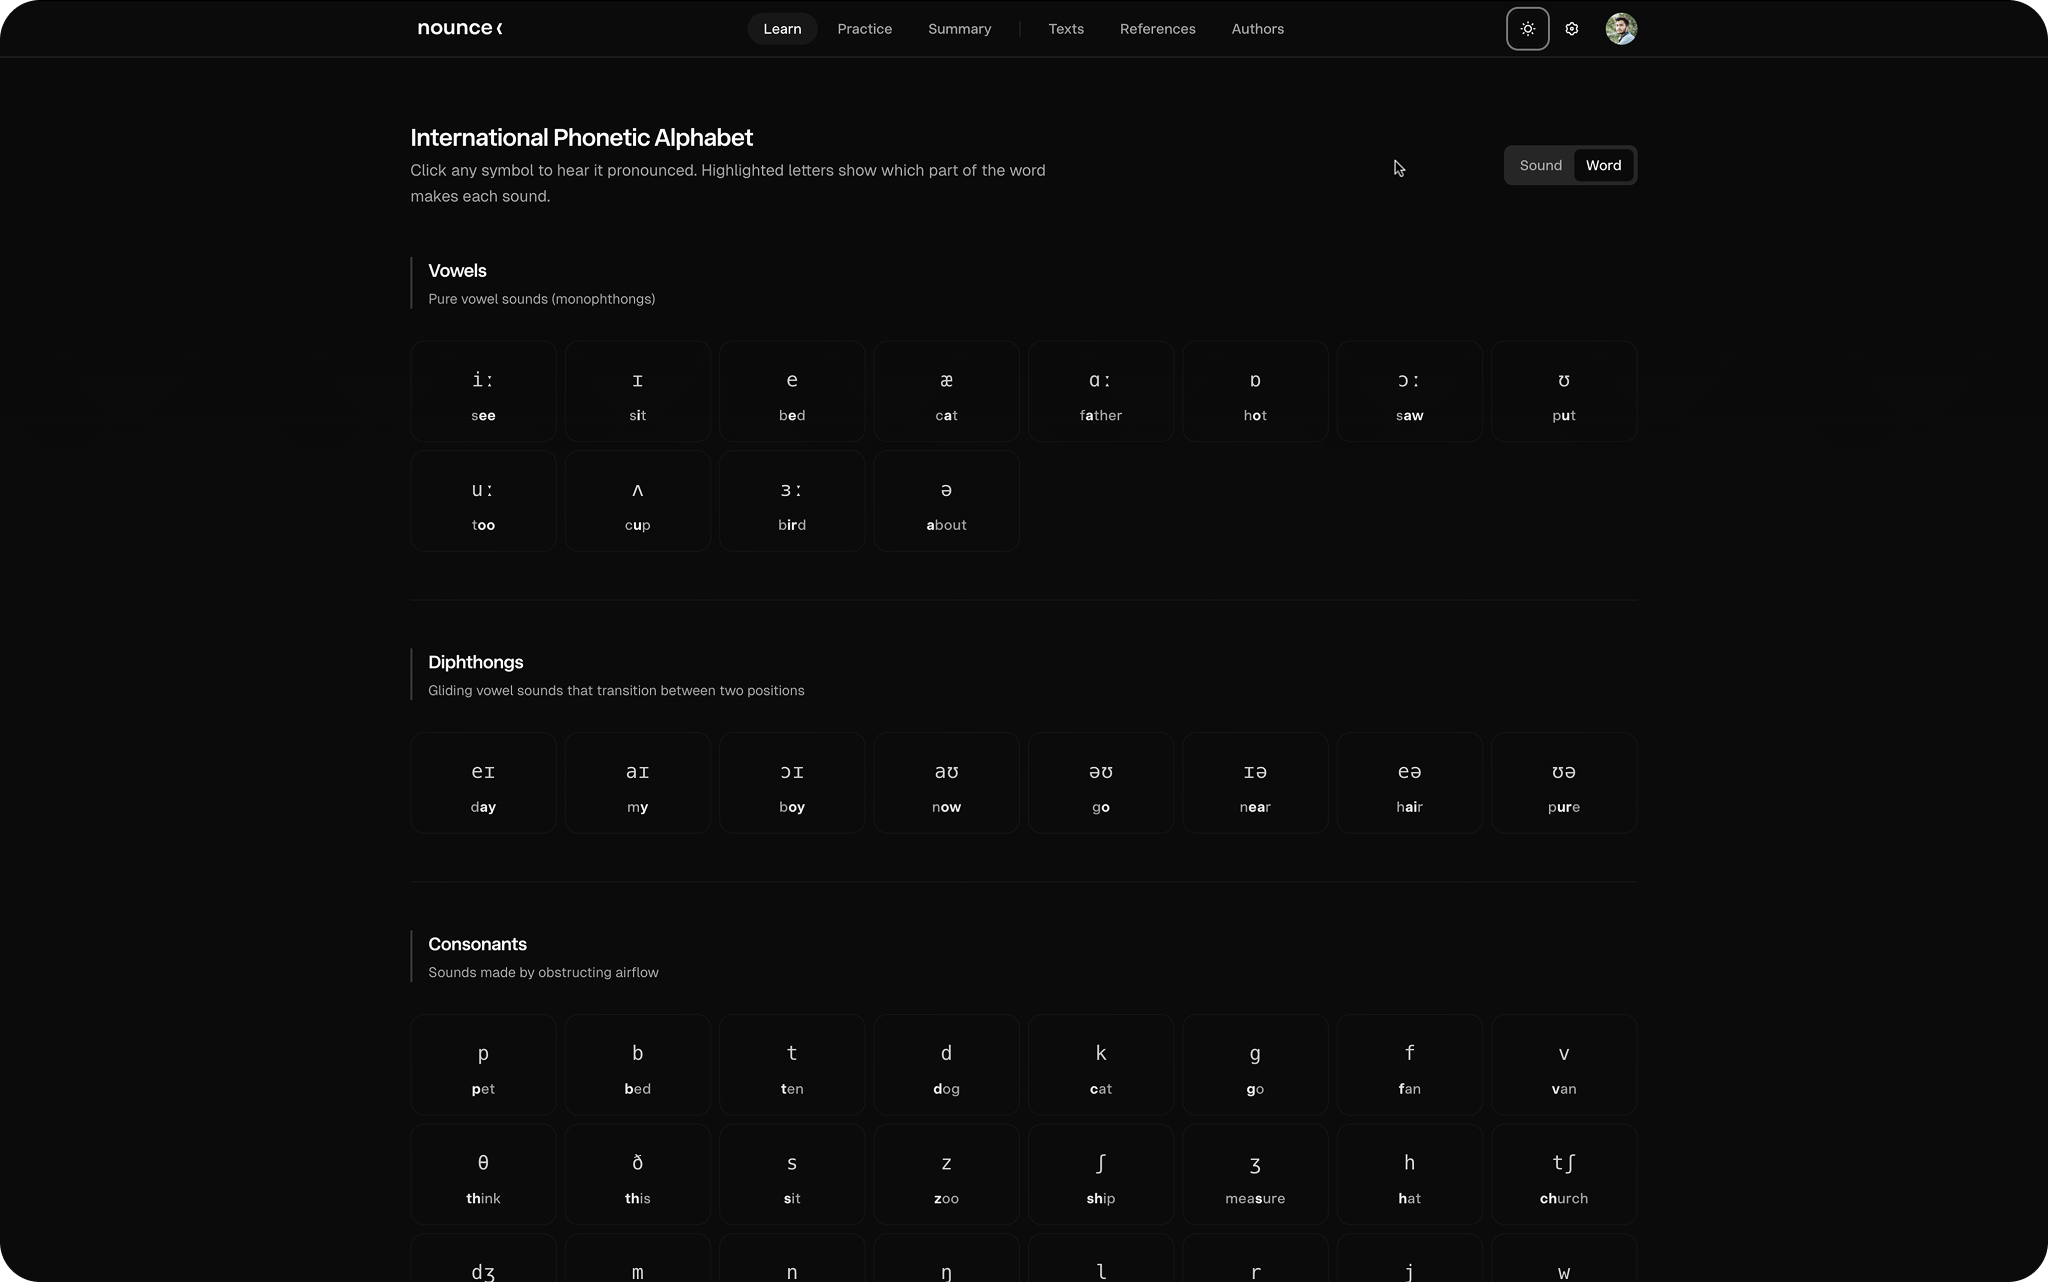
\includegraphics[width=\textwidth]{images/screen/nounce-ss-learn.png}
\caption{Educational Content - IPA and English phonology learning materials}
\label{fig:ui-learn}
\end{figure}

\subsubsection{Admin Interface}

\begin{figure}[H]
\centering
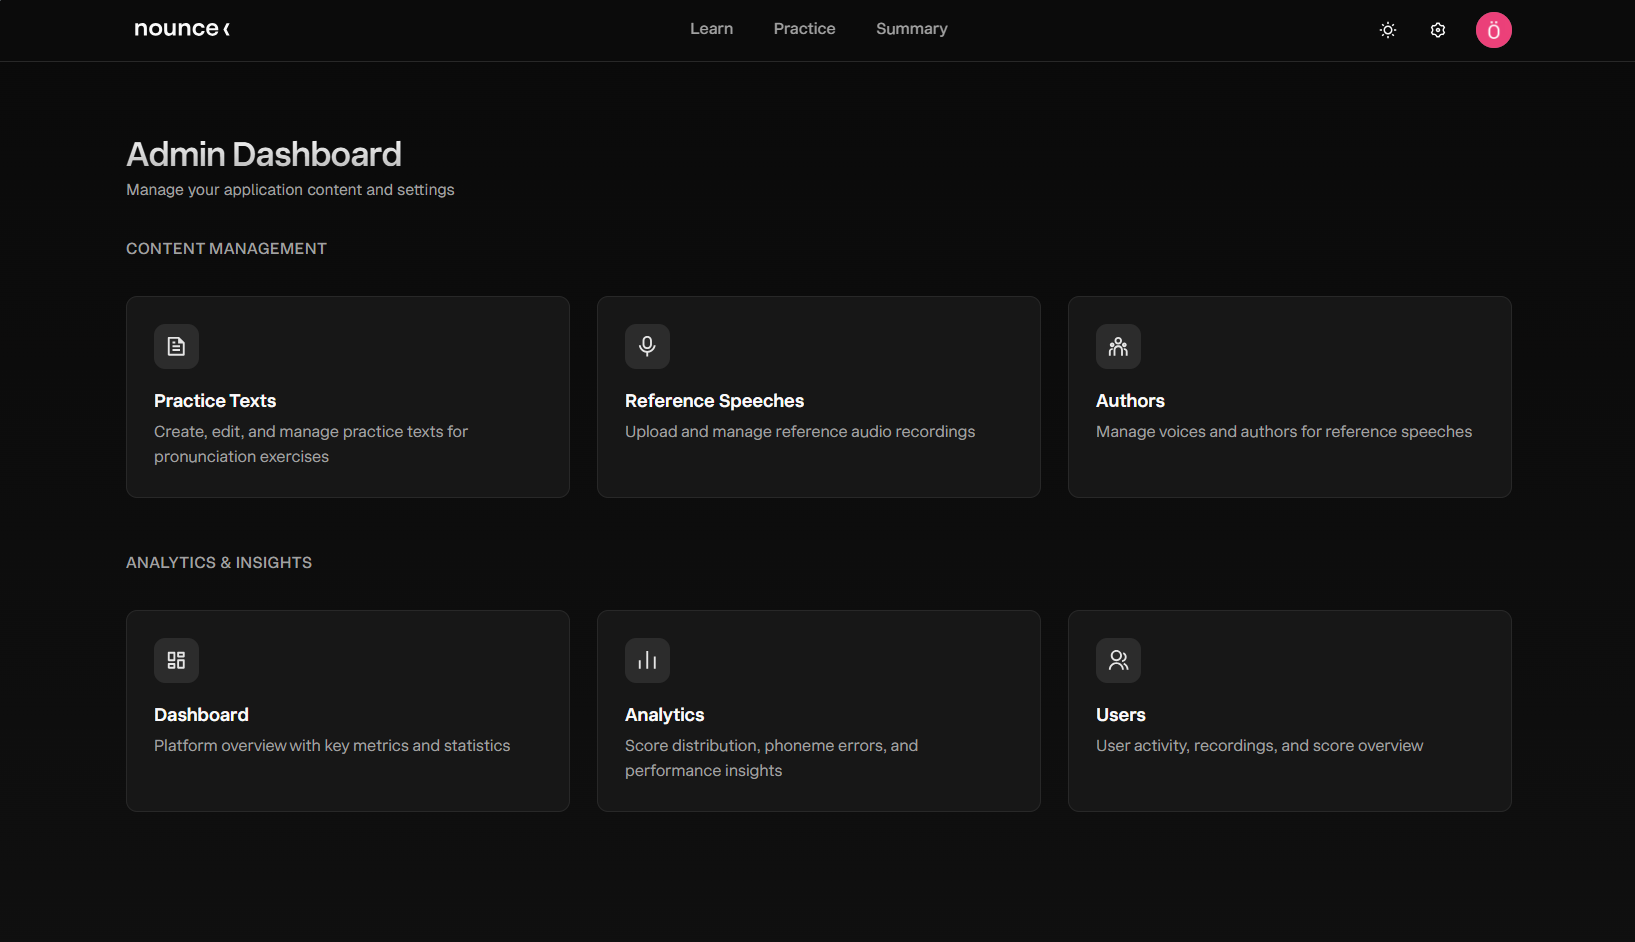
\includegraphics[width=\textwidth]{admin-img.png}
\caption{Admin Interface - Content management for practice texts and reference speeches}
\label{fig:ui-admin}
\end{figure}

\subsubsection{Mobile View}

\begin{figure}[H]
\centering
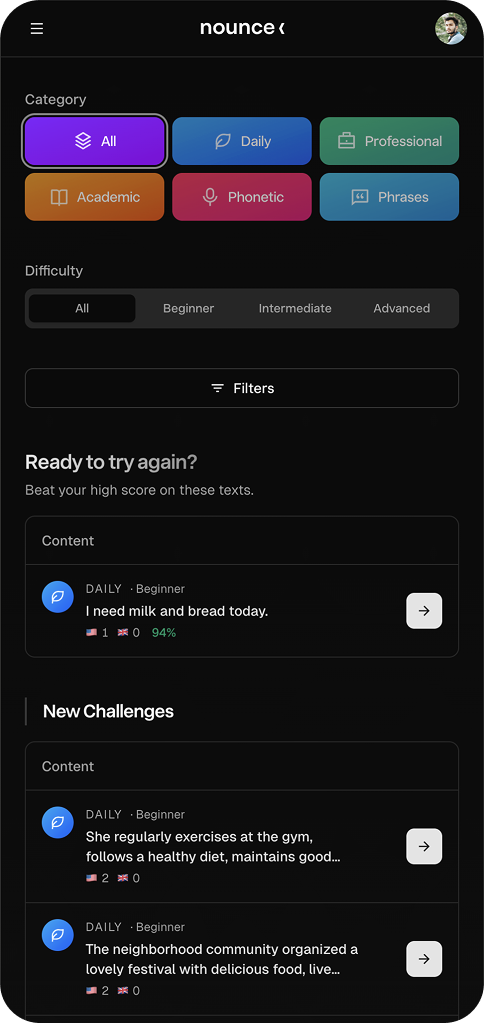
\includegraphics[width=0.6\textwidth]{images/screen/nounce-ss-mobile-view-practice.png}
\caption{Mobile View - Practice text selection on mobile devices}
\label{fig:ui-mobile}
\end{figure}


\chapter{IMPLEMENTATION AND TESTING}

\section{Implementation}

The implementation of Nounce follows the architecture and methodology outlined in previous chapters. The source code is organized in a structured repository \cite{github2024senior} with clear separation between the full-stack application, machine learning services, documentation, and experimental work.

\subsection{Full-Stack Application}

The main application codebase is located in the \texttt{app/} directory \cite{github2024app}, built with modern web technologies:

\textbf{Frontend:} The React-based user interface is implemented using TanStack Start for server-side rendering and routing. The UI follows modern design principles with Tailwind CSS, Shadcn UI, and ElevenLabs UI components, providing a sleek, responsive, and accessible experience across desktop and mobile devices. Key user-facing features include:
\begin{itemize}
    \item Practice text selection with filtering by difficulty (beginner, intermediate, advanced) and category (daily, professional, academic, phonetic challenge, common phrase)
    \item Browser-based audio recording with real-time waveform visualization
    \item Audio upload functionality with format conversion
    \item Pronunciation analysis results in a git-style diff viewer with goodness-of-pronunciation colour-coding, plus per-phone audio playback that highlights each phone as it is spoken
    \item Progress tracking and summary dashboard with statistics and error analysis
    \item Educational content pages for IPA and English phonology
\end{itemize}

\textbf{Backend:} The TanStack Start backend provides server functions for API endpoints and business logic. Authentication is handled through Clerk (free tier), supporting email/password and social sign-in options (Google, GitHub). Authorization is implemented using user metadata stored in Clerk, enabling role-based access control. The application uses TanStack Query for efficient data fetching, caching, and state management.

\textbf{Database:} The complete database schema is implemented using Drizzle ORM with Neon serverless PostgreSQL. All planned tables are operational, including:
\begin{itemize}
    \item \texttt{practice\_texts} - Practice materials with difficulty and category classification
    \item \texttt{authors} - Reference voice/author management (native General American and Received Pronunciation speakers)
    \item \texttt{reference\_speeches} - Target pronunciation audio files with IPA transcriptions
    \item \texttt{user\_recordings} - User-submitted audio recordings with metadata
    \item \texttt{audio\_quality\_metrics} - Quality assessment results (SNR, silence ratio, clipping ratio)
    \item \texttt{analyses} - Pronunciation assessment results with phoneme and word-level scores
    \item \texttt{alignments} - Legacy phone-level alignment table (V1; V2 stores phone timings directly on \texttt{reference\_speeches} and \texttt{analyses})
    \item \texttt{phoneme\_errors} and \texttt{word\_errors} - Normalized error data for aggregation
    \item \texttt{jobs} and \texttt{ipa\_generation\_jobs} - Asynchronous job tracking for RunPod endpoints
    \item \texttt{user\_preferences} - User settings and preferences
\end{itemize}

\textbf{Storage:} Audio files are stored in Cloudflare R2 object storage, with processed audio files (16-bit, 16kHz, mono WAV) maintained for long-term access. Metadata is stored in the PostgreSQL database with proper indexing for efficient queries.

\textbf{Admin Features:} Administrative interfaces are implemented for content management:
\begin{itemize}
    \item Practice text CRUD operations with bulk import capabilities
    \item Reference speech management with audio upload and IPA generation
    \item Author/voice management for native-speaker reference recordings
    \item Reference phone precomputation monitoring and management
\end{itemize}

Reference pronunciations are human native recordings in both General American and Received Pronunciation (commissioned voice talent), replacing the prototype's text-to-speech and letting learners choose a dialect to practise against.

\subsection{Machine Learning Services}

The machine learning pipeline is implemented as separate RunPod serverless endpoints in the \texttt{mod/} directory:

\textbf{Assessment Endpoint:} The pronunciation assessment service (\texttt{mod/assessment/}) is built around POWSM \cite{powsm} and its CTC encoder, and replaces several prototype components:
\begin{itemize}
    \item \textbf{Phone recognition:} POWSM CTC free alignment transcribes the IPA phones the learner actually produced, with real frame-level timestamps.
    \item \textbf{Forced alignment:} the reference phone sequence is force-aligned to the audio, also via POWSM's CTC path. This replaces the prototype's Montreal Forced Aligner and gives a single, consistent phone inventory across recognition and alignment instead of two tools with different inventories.
    \item \textbf{Audio-quality abstention:} a Silero voice-activity stage plus signal-quality checks (SNR, clipping) reject no-speech, noisy, or wrong-sentence recordings, returning an explained abstention rather than a misleading score.
    \item \textbf{Feature-aware difference:} produced and target phones are compared with an articulatory feature-vector distance (PanPhon) rather than exact-match edit distance, so a near-miss (e.g.\ a voicing-only swap) is treated as closer than a gross substitution. The same feature distance drives both the difference visualization and the learner-facing feedback.
    \item \textbf{Goodness-of-Pronunciation (GOP):} per-phone GOP and entropy are computed directly from the CTC posteriors, supporting confidence-aware, colour-coded feedback.
\end{itemize}

Because the reference phones are precomputed and supplied with each request, the GPU worker is stateless (it never re-aligns the reference). The endpoint is deployed on RunPod serverless GPU infrastructure, utilizing network volumes for model caching to minimize cold-start delays.

\textbf{Decommissioned G2P endpoint.} The prototype ran a separate Grapheme-to-Phoneme endpoint (\texttt{mod/ipa\_generation/}) to derive target IPA from text. This was removed in the present version: reference phones are computed once, offline, with the assessment model's own alignment, eliminating a second model load and a cross-model phone-inventory mismatch that had inflated error counts.

\subsection{Signal Processing and Experiments}

Signal processing experiments and deep learning model evaluations are conducted in the \texttt{sig/exp/} directory \cite{github2024sig}, which contains Jupyter notebooks for:
\begin{itemize}
    \item Audio preprocessing and quality assessment (SNR, silence detection, clipping detection)
    \item POWSM \cite{powsm} model evaluation and fine-tuning experiments
    \item POWSM CTC forced-alignment evaluation (replacing the prototype's MFA/TextGrid pipeline)
    \item Cross-dataset evaluation and comparison (L2-ARCTIC, speechocean762, and the in-house Turkish set)
    \item Visualization of phonetic features and alignment results
\end{itemize}

These notebooks document the experimentation process and serve as reference implementations for the production pipeline.

\subsection{Admin Analytics Dashboard}

An administrative analytics dashboard was developed to provide platform-wide insights and monitoring capabilities. The dashboard consists of three pages accessible from the admin interface:

\textbf{Overview Page:} Displays key platform metrics including total registered users, total analyses with status breakdown (completed, pending, processing, failed), practice text counts by difficulty level, reference speech count, platform-wide average pronunciation score, and audio quality distribution across accept, warning, and reject categories.

\textbf{Analytics Page:} Provides deeper analytical views using interactive charts built with the Recharts library. Features include a score distribution histogram showing the spread of pronunciation scores across five ranges, an area chart showing analysis activity over the past 30 days, ranked tables of the most common phoneme errors and phoneme confusion pairs (expected vs. actual), and processing time statistics (average, median, minimum, maximum).

\textbf{User Activity Page:} Presents a paginated table of all users with their recording counts, analysis counts, average scores, and last active timestamps, enabling administrators to monitor user engagement.

The dashboard is built using the same technology stack as the rest of the application: Drizzle ORM aggregation queries for data retrieval, TanStack Server Functions for the API layer, and TanStack Query for client-side data fetching and caching.

\subsection{User Progress and Summary Page}

A user-facing progress dashboard was implemented to help learners track their pronunciation improvement over time. The summary page provides:

\begin{itemize}
    \item \textbf{Statistics Overview:} Cards displaying total practice attempts, weekly attempt count with week-over-week progress percentage, and overall average pronunciation score.
    \item \textbf{Most Challenging Sounds:} An aggregated view of the user's most frequently missed phonemes, helping learners focus their practice on specific problem areas.
    \item \textbf{Practice History:} A filterable, paginated list of all practice attempts grouped by date (Today, Yesterday, Previous), with each entry showing the practice text, score, and timestamp. Users can filter by specific texts and sort by date or score.
\end{itemize}

The page requires authentication and displays a sign-in prompt for unauthenticated visitors.

\subsection{Documentation and Deployment}

The repository includes comprehensive documentation in the \texttt{doc/} directory, with learning materials, technical notes, database schema documentation, and project reports. The main README file \cite{github2024readme} provides an overview of the project structure, setup instructions, and development guidelines. Environment variables and configuration are documented to ensure reproducible deployments across different environments \cite{github2024env}.

The report build process is automated through \texttt{doc/report/build.sh}, which handles LaTeX compilation, bibliography processing, and diagram generation from PlantUML source files. The script integrates with \texttt{generate-diagrams.sh} to automatically generate all architecture and design diagrams before PDF compilation, ensuring documentation stays synchronized with code changes.

\section{Deployment}

Nounce is containerized using Docker, ensuring consistency across development, staging, and production environments. The deployment process is automated through GitHub Actions CI/CD pipelines \cite{github2024actions}, which handle building Docker images, running linting, running tests, and generating PlantUML diagrams from source files.

\subsection{Production Deployment}

The production application is deployed on Fly.io and served at \texttt{https://nounce.pro}. DNS management is handled through Cloudflare, which also provides DDoS protection via its global network infrastructure. The database is hosted on Neon serverless PostgreSQL, offering automatic scaling, point-in-time recovery, and branching capabilities. Audio files are stored in Cloudflare R2 object storage.

Machine learning services are deployed as RunPod serverless GPU endpoints, utilizing network volumes for model caching to reduce cold-start times. The deployment architecture is illustrated in Figure~\ref{fig:deployment-architecture}.

\subsection{Local Development}

For local development, a custom RunPod serverless simulator replicates the production API behavior without requiring cloud GPU resources. The simulator architecture, illustrated in Figure~\ref{fig:runpod-simulator}, consists of a FastAPI proxy server that mimics RunPod's job queue API, worker containers running locally via Docker Compose, and background async loops for job processing. The simulator is orchestrated using \texttt{docker-compose.dev.yml} and can be started using the \texttt{scripts/runpod.py} utility script.

The Docker configuration includes environment variable management and health checks for container monitoring. Building instructions, environment setup, and deployment procedures are documented in the repository README \cite{github2024readme}, with the build process automated through \texttt{doc/report/build.sh} script that handles LaTeX compilation and diagram generation.

\chapter{RESULTS}

This chapter presents the results achieved in the development of Nounce, including technical achievements, system capabilities, implementation status, and model evaluation findings.

\section{POWSM-CTC Evaluation Results}

The POWSM-CTC variant (\texttt{espnet/owsm\_ctc\_v3.1\_1B}) was evaluated on three test recordings from two Turkish-native English speakers reading English sentences. The results are summarized in Table~\ref{table:ctcResults}.

\begin{table}[htbp]
\vskip\baselineskip
\caption[POWSM-CTC evaluation results]{POWSM-CTC evaluation results on Turkish-native English speaker recordings.}
\begin{center}
\begin{tabular}{|c|c|c|c|c|} \hline
\textbf{Sample} & \textbf{PR Phones} & \textbf{G2P Phones} & \textbf{Total Errors} & \textbf{Error Types} \\\hline
umit12 & 86 & 0 & 86 & 86 insertions \\\hline
yusuf12 & 83 & 0 & 83 & 83 insertions \\\hline
umit14 & 91 & 0 & 91 & 91 insertions \\\hline
\textbf{Average} & \textbf{86.7} & \textbf{0} & \textbf{86.7} & \textbf{100\% insertions} \\\hline
\end{tabular}
\label{table:ctcResults}
\end{center}
\end{table}

The G2P task produced empty transcriptions for all test samples, as the CTC encoder-only architecture lacks the decoder component required for text-conditioned phoneme generation. Consequently, all phonemes detected by Phone Recognition were classified as insertion errors, rendering the assessment scores meaningless. These results confirmed that the encoder-decoder POWSM architecture is necessary for the pronunciation assessment pipeline, where both PR and G2P tasks must operate on a consistent phone inventory with reliable text-conditioned output.

\section{Fine-Tuning Evaluation and Validation Study}
\label{sec:finetuning-results}

This section presents the empirical centerpiece of the project: the annotation-convention ablation (Section~\ref{sec:finetuning-method}), a human-judgment validation study, and an external benchmark validation.

\subsection{Annotation-Convention Ablation (Canonical vs.\ Perceived)}

Table~\ref{table:ftAblation} compares the baseline POWSM against the canonical- and perceived-label adapters at both training budgets. The clinically relevant metric is \emph{deviation recall} on L2-ARCTIC: the fraction of annotated canonical$\rightarrow$produced substitutions the model actually reproduces (rather than normalizing away). Higher PER/recall figures use the same phone-folding convention on both sides so the comparison reflects phone identity rather than diacritic differences.

\begin{table}[htbp]
\vskip\baselineskip
\caption[Annotation-convention fine-tuning ablation]{Canonical vs.\ perceived fine-tuning, 30 vs.\ 60 epochs. TR = Turkish-native held-out set; L2A = L2-ARCTIC held-out dev set. Native FPR is drift on correct native speech (lower is better).}
\begin{center}
\begin{tabular}{|l|c|c|c|c|c|} \hline
\textbf{Model} & \textbf{TR-PER} & \textbf{TR sub-rec.} & \textbf{Native FPR} & \textbf{L2A PER/PPL} & \textbf{L2A dev-rec.} \\\hline
base POWSM & 0.435 & 0.033 & 0.003 & 0.240 & 0.173 \\\hline
\texttt{l2a\_cpl} (30ep) & 0.426 & 0.016 & 0.007 & 0.238 & 0.173 \\\hline
\texttt{l2a\_cpl\_long} (60ep) & 0.400 & 0.008 & 0.027 & 0.217 & \textbf{0.163} \\\hline
\texttt{l2a\_ppl} (30ep) & 0.420 & 0.025 & 0.008 & 0.227 & 0.186 \\\hline
\texttt{l2a\_ppl\_long} (60ep) & \textbf{0.392} & \textbf{0.057} & 0.024 & \textbf{0.205} & \textbf{0.213} \\\hline
\end{tabular}
\label{table:ftAblation}
\end{center}
\end{table}

The result confirms the hypothesis, and sharpens with training budget. At 30 epochs the canonical adapter is a \emph{no-op}: \texttt{l2a\_cpl} matches the baseline's deviation recall exactly ($0.173$), because the base model already emits canonical-leaning phones and canonical supervision teaches it nothing new. At 60 epochs the canonical adapter \emph{actively harms}: \texttt{l2a\_cpl\_long} deviation recall drops \emph{below} base ($0.163 < 0.173$) as the model normalizes harder and loses produced deviations. The perceived adapter moves in the opposite direction: \texttt{l2a\_ppl\_long} reaches $0.213$ deviation recall and is the only model to beat base on both Turkish PER ($0.392$) and Turkish substitution recall ($0.057$ vs.\ $0.033$). The cpl-vs-ppl gap widens roughly four-fold between the two budgets---identical audio, opposite supervision, diverging behaviour. The cost of the longer schedule is increased native drift (FPR $0.024$ vs.\ $0.003$ for base); \texttt{l2a\_ppl\_long} is deployed as the production model, accepting this drift for materially better learner-deviation detection. The LOSO arm (adding three Turkish speakers) gives a modest, high-variance speaker-independent gain (mean PER $0.421$, range $0.402$--$0.455$).

% TODO: replace the [TODO] figure placeholders below with the rendered PNGs from
% artifacts/eval/figs/ (copy them into doc/report/images/). cpl_vs_ppl.png and
% l2arctic_cpl_vs_ppl.png are the headline figures.
\textbf{[TODO: insert figure \texttt{artifacts/eval/figs/l2arctic\_cpl\_vs\_ppl.png} (per-L1 deviation recall, cpl vs ppl) into \texttt{doc/report/images/}.]}

\subsection{Human-Judgment Validation}

To assess whether the system's pronunciation score tracks human perception, native English raters score each Turkish-learner clip for intelligibility (0--10) through a blind rating interface (Figure~\ref{fig:intelligibility-ui}), and we correlate the mean human rating against the system score via Spearman's $\rho$. With two raters and 24 jointly-scored clips, $\rho = 0.37$ between the system score and the mean human rating---a positive but only moderate association, visible as a loose upward trend in Figure~\ref{fig:scatter-system-human}.

\begin{figure}[H]
\centering
% TODO: capture a screenshot of the /intelligibility-score blind rating page and
% save it to doc/report/images/screen/nounce-ss-intelligibility.png, then replace
% the fbox below with: 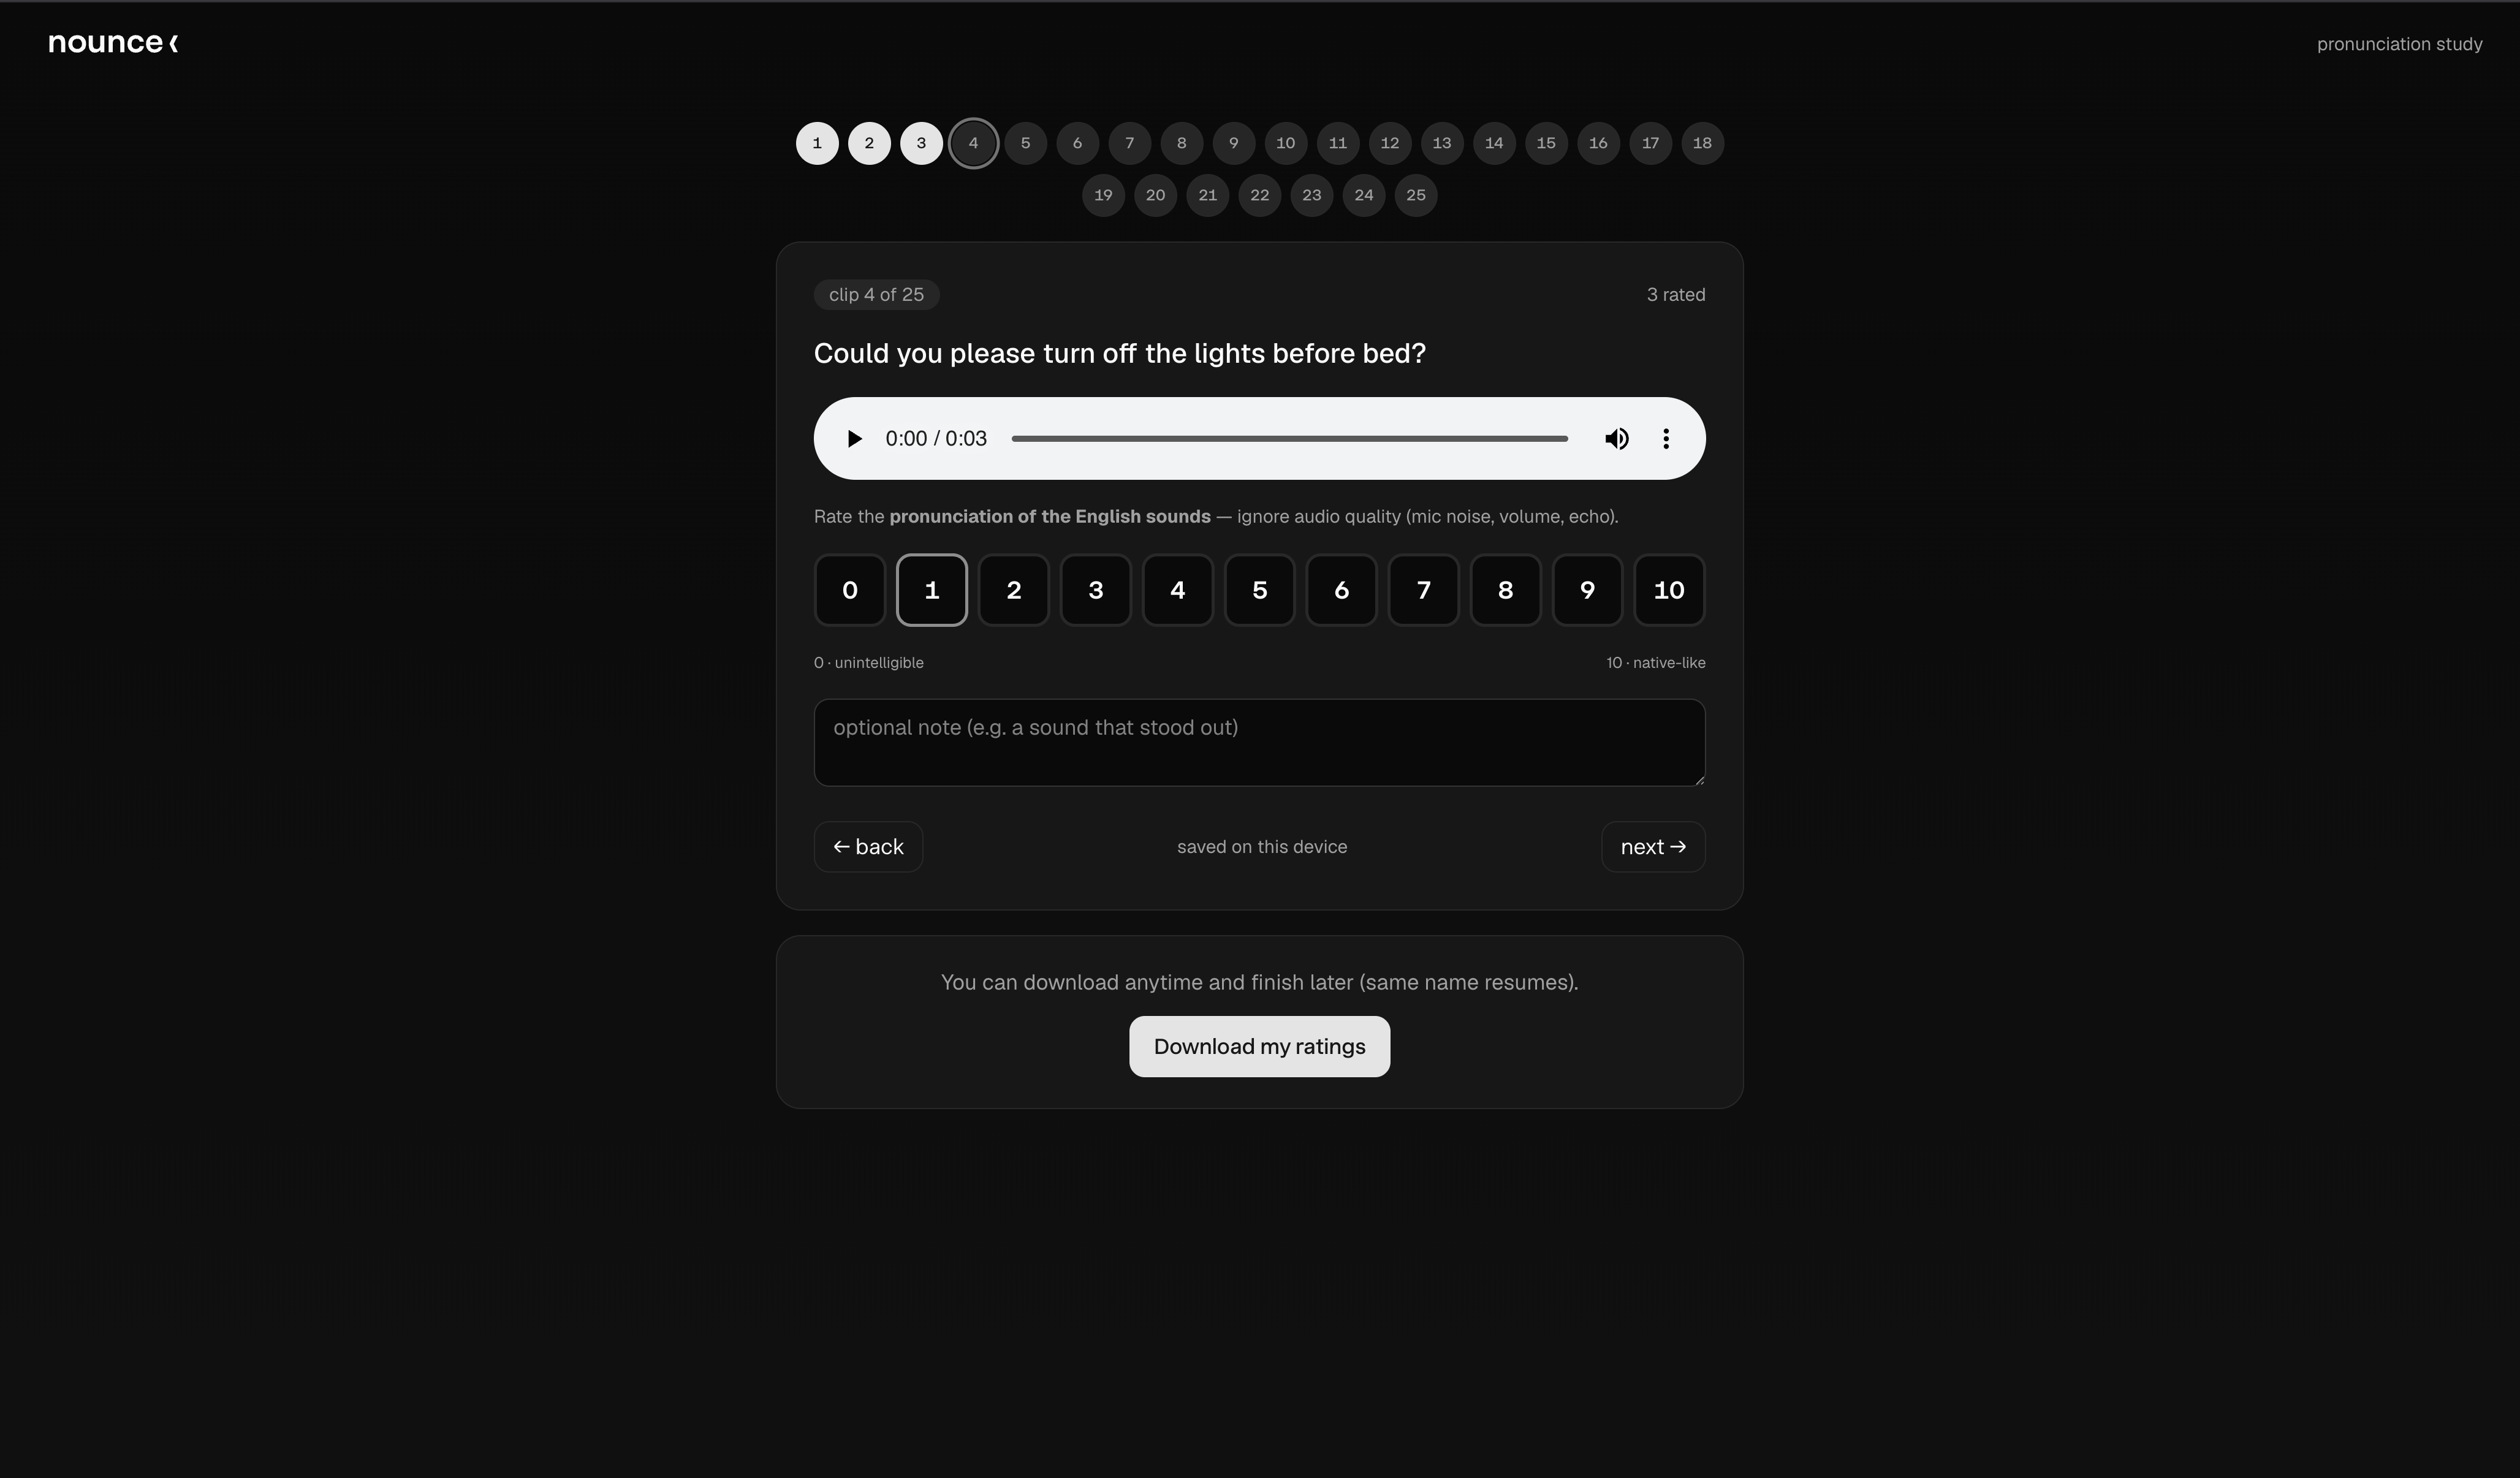
\includegraphics[width=\textwidth]{images/screen/nounce-ss-intelligibility.png}
\fbox{\parbox[c][6cm][c]{0.9\textwidth}{\centering \textbf{[TODO: app screenshot]}\\ Blind intelligibility-rating interface (\texttt{/intelligibility-score}): per-clip 0--10 scale, progress dots, audio playback.}}
\caption{The blind human-rating interface used in the validation study.}
\label{fig:intelligibility-ui}
\end{figure}

The two raters themselves agree only weakly, however: their pairwise Spearman correlation is $0.16$ and Krippendorff's $\alpha$ (interval metric) is $0.11$, far below the $0.667$ threshold conventionally taken as a floor for tentative reliability. This is the more important finding of the study in its current form. Intelligibility is a genuinely subjective judgment, and with only two raters over a small clip set the human ``ground truth'' is itself noisy; a system-vs-human correlation cannot exceed what the humans share with each other. We therefore read $\rho = 0.37$ as encouraging but preliminary evidence that the score points in the right direction, not as a validated agreement figure. The clear next step---and the chief bottleneck for substantiating the system's pedagogical claims---is to recruit more raters (so the mean human rating stabilizes and $\alpha$ becomes interpretable) and to broaden the clip set beyond a single speaker. The analysis is fully scripted (\texttt{sig/analysis/validation.py}, pure-stdlib statistics) and re-runs automatically as additional rater submissions land, so this figure is expected to firm up without further engineering.

\begin{figure}[H]
\centering
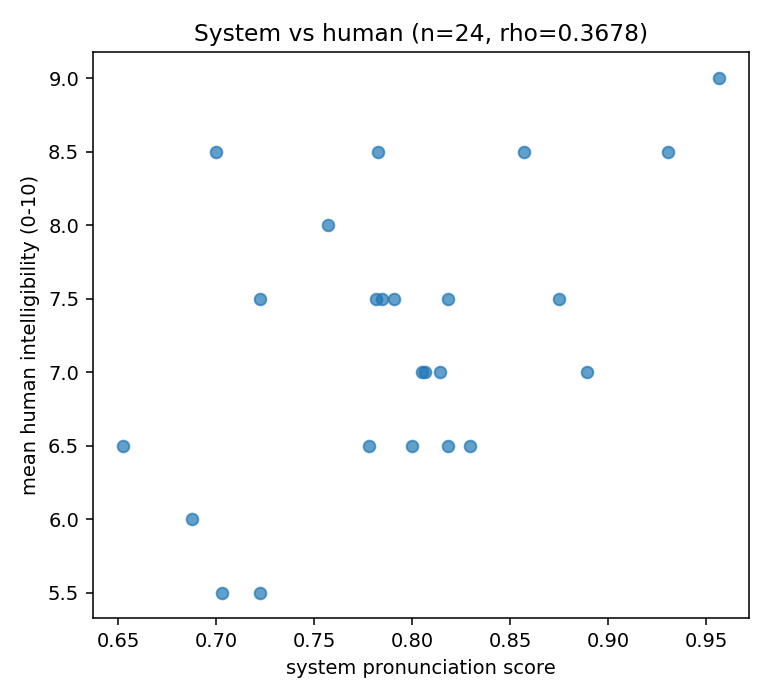
\includegraphics[width=0.6\textwidth]{figures/scatter_system_vs_human.png}
\caption[System score vs.\ mean human intelligibility]{System pronunciation score against mean human intelligibility rating (0--10) across the 24 jointly-rated clips. Spearman's $\rho = 0.37$. The loose upward cloud reflects both a real positive association and the weak inter-rater agreement ($\alpha = 0.11$) that bounds it.}
\label{fig:scatter-system-human}
\end{figure}

\subsection{External Benchmark Validation (speechocean762)}

As an independent, large-scale check, we evaluate the system's Goodness-of-Pronunciation (GOP) score against expert human phoneme-accuracy labels on the standard speechocean762 benchmark \cite{speechocean762} (2{,}500 held-out utterances, 47{,}369 phones, Mandarin-L1). Mean GOP rises monotonically with the human accuracy label ($-6.80$, $-4.65$, $-1.37$ for accuracy $0$, $1$, $2$), and Spearman's $\rho$ is $0.21$ at the phone level and $0.37$ at the sentence level. This confirms, on a recognized public benchmark and a different L1, that the GOP component tracks human pronunciation judgment; it complements (rather than replaces) the Turkish-specific study.

\textbf{[TODO: insert the GOP-vs-accuracy box plot \texttt{artifacts/speechocean/figs/gop\_vs\_accuracy.png}.]}

\subsection{Scaling the Perceived-Label Fine-Tune to Full L2-ARCTIC}

The full-corpus perceived-label fine-tune described in Section~\ref{sec:finetuning-method} applies the same convention to a held-out population roughly an order of magnitude larger than the controlled dev split. Evaluated on its own protocol---a six-L1, speaker-disjoint test set ($\approx$900 utterances), greedy decoding, and raw PER against the perceived labels---the adapter lowers phone error rate from a baseline of $0.388$ to $0.192$, a $19.5$~percentage-point reduction that holds in \emph{every one} of the six first-language groups (Table~\ref{table:l2aFullPerL1}). On this protocol the per-phone breakdown moves in the expected direction, with the largest error reductions on exactly the segments that distinguish L2 from native English---the American rhotic ``r'', the reduced schwa, the lax vowels of \emph{bit} and \emph{cat}, and the glide ``w''. Read at face value this is a strong, uniform gain; the qualification below is that the gain does not transfer cleanly to the project's stricter, folding-aware evaluation.

\begin{table}[h]
\centering
\caption[Full L2-ARCTIC perceived-label fine-tune, per-L1 PER]{Per-L1 phone error rate (vs.\ perceived labels) for the full-corpus perceived-label fine-tune, baseline POWSM vs.\ the perceived-label LoRA adapter, on the six-L1 speaker-disjoint test set. Greedy decoding; PER measured without diacritic folding (see text).}
\label{table:l2aFullPerL1}
\begin{tabular}{|l|c|c|c|} \hline
\textbf{First language} & \textbf{Baseline PER} & \textbf{Perceived-LoRA PER} & \textbf{$\Delta$ (pp)} \\\hline
Arabic     & 0.362 & 0.167 & $-19.4$ \\\hline
Hindi      & 0.331 & 0.181 & $-15.0$ \\\hline
Korean     & 0.404 & 0.208 & $-19.6$ \\\hline
Mandarin   & 0.387 & 0.207 & $-18.1$ \\\hline
Spanish    & 0.382 & 0.174 & $-20.9$ \\\hline
Vietnamese & 0.459 & 0.218 & $-24.1$ \\\hline
\textbf{Overall} & \textbf{0.388} & \textbf{0.192} & $\mathbf{-19.5}$ \\\hline
\end{tabular}
\end{table}

Table~\ref{table:l2aFullPerL1} is measured on the full-corpus run's own protocol---its $\approx$900-utterance six-L1 test split, greedy decoding, and raw (unfolded) PER against the labels the adapter was trained to emit. To place this adapter on the same axis as the controlled ablation, we also scored it through the project's standard harness (folded phone identity, free recognition, the held-out Turkish set, the 600-utterance L2-ARCTIC dev split, and the native-drift probe), exactly as for \texttt{l2a\_ppl\_long}. On those shared metrics the picture is more nuanced (Table~\ref{table:l2aFullShared}). The full-corpus adapter attains the \emph{highest} deviation recall of any model we trained ($0.362$, more than double the baseline's $0.173$) and the highest Turkish substitution recall ($0.131$); it is unambiguously the most sensitive deviation detector. But that sensitivity comes from transcribing aggressively: on the standard dev split its phone error rate against the perceived labels \emph{rises} above baseline ($0.328$ vs.\ $0.240$), per-phone error counts grow rather than shrink on the dominant vowels (lax-i $273 \rightarrow 951$, the \emph{book} vowel $106 \rightarrow 472$), and---most consequentially for a deployed system---its native false-positive rate reaches $0.203$, meaning it would flag roughly one in five \emph{correctly} pronounced native phones as an error.

\begin{table}[h]
\centering
\caption[Full-corpus adapter on the shared evaluation axis]{The full-corpus adapter (\texttt{l2a\_ppl\_full}) scored through the project's standard harness, alongside the baseline and the deployed \texttt{l2a\_ppl\_long}, so all three sit on one axis (cf.\ Table~\ref{table:ftAblation}). TR = Turkish-native held-out set; L2A = L2-ARCTIC dev set; native FPR is drift on correct native speech (lower is better).}
\label{table:l2aFullShared}
\begin{tabular}{|l|c|c|c|c|c|} \hline
\textbf{Model} & \textbf{TR-PER} & \textbf{TR sub-rec.} & \textbf{Native FPR} & \textbf{L2A PER/PPL} & \textbf{L2A dev-rec.} \\\hline
base POWSM & 0.435 & 0.033 & 0.003 & 0.240 & 0.173 \\\hline
\texttt{l2a\_ppl\_long} (deployed) & \textbf{0.392} & 0.057 & 0.024 & \textbf{0.205} & 0.213 \\\hline
\texttt{l2a\_ppl\_full} & 0.432 & \textbf{0.131} & 0.203 & 0.328 & \textbf{0.362} \\\hline
\end{tabular}
\end{table}

The two evaluations of the same adapter therefore diverge, and the divergence is itself informative. On its own protocol the full-corpus run shows a large, uniform PER improvement; on the shared, folding-aware protocol with a native-drift probe it reads as a high-recall, low-precision detector that over-fires. Both readings are consistent with the central convention claim---perceived-label supervision teaches the model to surface produced deviations rather than normalize them---but they part company on \emph{deployability}. A pronunciation tutor that mislabels a fifth of correct native speech would erode user trust, so the deployed model remains \texttt{l2a\_ppl\_long}, which captures most of the deviation-detection gain (recall $0.213$ vs.\ base $0.173$, and the best Turkish PER of any adapter) at a native false-positive rate an order of magnitude lower ($0.024$ vs.\ $0.203$). The full-corpus adapter is retained as an evaluation reference that maps the recall-versus-precision frontier, not as a production candidate. The practical lesson reinforces the thesis from a new direction: the supervision convention determines \emph{whether} a model detects deviations, but the training budget and corpus breadth govern \emph{how aggressively}---and a usable tutor must sit on the conservative side of that trade-off.

\section{System Implementation Status}

The Nounce pronunciation assessment system has been successfully implemented with the following components operational:

\subsection{Full-Stack Web Application}

The complete web application is functional and deployed, providing users with a comprehensive pronunciation assessment platform. The system successfully implements:

\begin{itemize}
    \item \textbf{User Authentication:} Secure authentication through Clerk with support for email/password and social sign-in (Google, GitHub)
    \item \textbf{Practice Text Management:} Full CRUD operations for practice texts with filtering by difficulty and category
    \item \textbf{Audio Recording:} Browser-based recording with real-time waveform visualization and audio upload support
    \item \textbf{Reference Speech System:} Management of target pronunciations as human native recordings (General American and Received Pronunciation), with a learner-facing dialect toggle (the prototype's TTS generation was retired)
    \item \textbf{Pronunciation Assessment:} End-to-end workflow from recording to detailed analysis results
    \item \textbf{Progress Tracking:} User history, statistics, and error analysis with aggregation capabilities
    \item \textbf{Admin Interface:} Complete administrative tools for content and system management
\end{itemize}

\subsection{Database Schema}

The complete database schema is implemented and operational, with all planned tables, relationships, and indexes in place. The schema supports:
\begin{itemize}
    \item User recordings with metadata and quality metrics
    \item Pronunciation analyses with phoneme and word-level scoring
    \item Error tracking with normalized data for aggregation
    \item Asynchronous job processing with status tracking
    \item Reference speech management with IPA transcriptions
    \item User preferences and progress data
\end{itemize}

\subsection{Machine Learning Pipeline}

The machine learning assessment pipeline is fully integrated:

\begin{itemize}
    \item \textbf{POWSM Integration:} Successfully integrated POWSM \cite{powsm} models for Phone Recognition (PR) and Grapheme-to-Phoneme (G2P) tasks
    \item \textbf{Phonetic Transcription:} Accurate IPA transcription from audio using state-of-the-art models
    \item \textbf{Error Detection:} Phoneme-level error classification (substitution, insertion, deletion) with edit distance algorithms
    \item \textbf{Time Alignment:} POWSM CTC forced alignment for phone-level timestamps (replacing the prototype's MFA)
    \item \textbf{Score Calculation:} Pronunciation accuracy scoring based on error rates
\end{itemize}

The assessment endpoint processes audio recordings and returns detailed analysis including:
\begin{itemize}
    \item Actual IPA transcription from user speech
    \item Target IPA transcription from reference text
    \item Overall pronunciation score (0.0-1.0)
    \item Phoneme-level error list with timestamps
    \item Word-level error analysis
\end{itemize}

\subsection{Audio Quality Assessment}

Audio quality metrics are calculated and stored for each user recording:
\begin{itemize}
    \item Signal-to-Noise Ratio (SNR) in decibels
    \item Silence ratio (percentage of quiet segments)
    \item Clipping ratio (percentage of clipped samples)
    \item Noise ratio (percentage of noise segments)
    \item Quality status classification (accept, warning, reject)
\end{itemize}

Quality thresholds are applied at the application layer, allowing flexible adjustment without database migrations.

\subsection{Deployment Infrastructure}

The system is deployed using modern cloud infrastructure:
\begin{itemize}
    \item \textbf{Domain:} The application is served at \texttt{https://nounce.pro}, with the domain purchased and configured for production use
    \item \textbf{DNS and Security:} DNS management and DDoS protection are handled through Cloudflare's global network infrastructure
    \item \textbf{Application Hosting:} Docker containerized application deployed on Fly.io with global edge deployment
    \item \textbf{Database:} Neon serverless PostgreSQL with automatic scaling and backups
    \item \textbf{Object Storage:} Cloudflare R2 for audio file storage
    \item \textbf{ML Services:} RunPod serverless endpoints for GPU-powered inference
    \item \textbf{CI/CD:} GitHub Actions pipelines for automated testing and deployment
\end{itemize}

\section{Technical Achievements}

\subsection{Architecture and Design}

The system demonstrates a well-architected full-stack application with:
\begin{itemize}
    \item Clear separation of concerns between frontend, backend, database, and ML services
    \item Type-safe database operations using Drizzle ORM with TypeScript
    \item Modern React patterns with server-side rendering and efficient data fetching
    \item Scalable serverless architecture supporting concurrent users
    \item Comprehensive error handling and user feedback mechanisms
\end{itemize}

\subsection{User Experience}

The application provides an intuitive and responsive user experience:
\begin{itemize}
    \item Modern, accessible UI following web standards and best practices
    \item Real-time feedback during recording and processing
    \item Clear visualization of pronunciation errors with IPA highlighting
    \item Progress tracking with historical data and statistics
    \item Mobile-responsive design supporting multiple devices
\end{itemize}

\subsection{Integration Challenges and Solutions}

Several technical challenges were successfully addressed during implementation:

\textbf{Model Integration:} Integrating POWSM \cite{powsm} models required extensive experimentation due to limited documentation. The solution involved custom implementation of model loading, inference pipelines, and output parsing.

\textbf{Audio Processing:} Handling various audio formats and quality levels required robust preprocessing pipelines. The system implements format conversion, quality assessment, and normalization to ensure consistent input for ML models.

\textbf{Asynchronous Processing:} Managing long-running ML inference tasks required a job queue system. The implementation uses RunPod's serverless architecture with status tracking and webhook callbacks for result delivery.

\textbf{Time Alignment:} Phone-level timestamps come directly from POWSM's CTC forced alignment, computed on the same encoder used for recognition. This replaced the prototype's MFA/TextGrid pipeline and its heuristic fallback timestamps, removing a separate tool, a separate phone inventory, and a class of alignment mismatches.

\section{Performance and Scalability}

The system architecture supports scalability and demonstrates good performance characteristics:
\begin{itemize}
    \item Serverless database (Neon) with automatic scaling
    \item Object storage (Cloudflare R2) for efficient audio file management
    \item RunPod GPU endpoints for parallel ML inference with network volume caching
    \item Job queue system for handling concurrent assessment requests
    \item Efficient database indexing for fast queries
\end{itemize}

\textbf{Performance Metrics:}
\begin{itemize}
    \item Average Phone Recognition (PR) task execution time: 3 seconds
    \item Average Grapheme-to-Phoneme (G2P) task execution time: 2 seconds
    \item Maximum observed cold-start time: 30 seconds (first request after inactivity)
    \item Subsequent requests benefit from cached models in network volumes, eliminating cold-start delays
\end{itemize}

These performance characteristics enable responsive user experience while maintaining cost efficiency through serverless GPU infrastructure that scales to zero when not in use.

\chapter{CONCLUSION}

This project successfully developed Nounce, a comprehensive web-based pronunciation assessment system for English language learners. The system integrates state-of-the-art machine learning models, modern web technologies, and pedagogical principles to provide detailed, actionable feedback on pronunciation accuracy.

\section{Project Summary}

Nounce addresses the critical need for accessible pronunciation learning tools by providing:
\begin{itemize}
    \item \textbf{Phonetic-Level Analysis:} Detailed pronunciation assessment at the phoneme level using the International Phonetic Alphabet (IPA)
    \item \textbf{Automated Feedback:} Instant, judgment-free feedback on pronunciation errors with clear visualization
    \item \textbf{Educational Integration:} Guidance on English phonology concepts to help learners understand and improve
    \item \textbf{Progress Tracking:} Historical analysis and statistics to monitor improvement over time
    \item \textbf{Accessible Design:} Web-based platform accessible from any device without requiring native speaker tutors
\end{itemize}

\section{Technical Contributions}

The project demonstrates several technical achievements:

\textbf{Model Integration:} Successfully integrated POWSM \cite{powsm} (Phonetic Open Whisper-Style Speech Model), a state-of-the-art phonetic transcription model, for accurate phone recognition and grapheme-to-phoneme conversion. The integration required custom implementation due to limited documentation, contributing to the open-source community's understanding of these models.

\textbf{Full-Stack Architecture:} Developed a production-ready full-stack application using modern technologies (TanStack Start, React, TypeScript, Drizzle ORM) with a focus on type safety, scalability, and maintainability. The architecture demonstrates best practices in separation of concerns, error handling, and user experience design.

\textbf{ML Pipeline:} Implemented a complete machine learning pipeline combining POWSM CTC phonetic transcription and forced alignment, audio-quality abstention, articulatory feature-vector difference, and GOP scoring. The pipeline processes audio recordings asynchronously and provides detailed analysis results with real CTC phone-level timestamps.

\textbf{Database Design:} Designed and implemented a comprehensive database schema supporting user recordings, analyses, error tracking, and progress data. The schema enables efficient querying and aggregation for analytics and reporting.

\section{Educational Impact}

Nounce contributes to language learning by:
\begin{itemize}
    \item Providing 24/7 access to pronunciation assessment without requiring human tutors
    \item Offering detailed, phonetic-level feedback that helps learners understand specific sound production issues
    \item Creating a safe, judgment-free environment for practice
    \item Supporting self-directed learning with progress tracking and historical analysis
    \item Introducing learners to IPA and phonetic concepts, building domain knowledge
\end{itemize}

The system acknowledges that it does not replace human-to-human interaction in language learning, but rather serves as a supplementary tool for learners who may lack access to native speakers or formal language education resources.

\section{Conclusion and Future Work}

\subsection{State of the Platform}

All core features are functional, and the application is deployed. The system provides a complete pronunciation assessment workflow from recording to detailed feedback, with administrative tools for content management. Additional content management and data curation is still needed for future expansion.

\subsection{Limitations}

All core features are functional, and the application is deployed. Additional content management and data curation is still needed for future expansion to support a broader range of practice materials and user populations.

The POWSM \cite{powsm} model operates in a hybrid space between phonemic and phonetic representation, which can introduce occasional inaccuracies. The model's output may not always perfectly align with canonical IPA transcriptions, particularly for non-standard pronunciations or regional variations.

Nounce is designed exclusively for English to streamline initial development and ensure high-quality pronunciation assessment. Future development can expand support to additional languages, but this requires significant model adaptation, dictionary resources, and acoustic model training for each target language.

\subsection{Future Directions}

\textbf{Scaling the Turkish-L1 adaptation:} This work already fine-tuned POWSM for Turkish-native speakers and showed that perceived-label adaptation improves mispronunciation detection (Section~\ref{sec:finetuning-results}). The clearest next step is to scale the perceived-annotated Turkish data well beyond the current small set---the chief bottleneck being expert phonetic annotation in the model's convention---and to reduce the native-speech drift introduced by longer fine-tuning. Broadening the human-rating validation (more raters and speakers) is the other resource-bound priority, since it is what most directly substantiates the system's pedagogical claims.

\textbf{Language Expansion:} Nounce is designed exclusively for English to streamline initial development and ensure high-quality pronunciation assessment. Future development can expand support to additional languages, but this requires significant model adaptation, dictionary resources, and acoustic model training for each target language.

\textbf{Voice Cloning:} Leverage voice cloning technology to generate target pronunciations with the user's voice for personalized feedback. This would allow learners to hear correct pronunciations in their own voice, potentially improving comprehension and retention.

\textbf{LLM Analysis:} Integrate a Large Language Model (LLM) to analyze performance data and provide user-specific, targeted feedback on each attempt, aggregated over time. The LLM could identify patterns in errors, suggest personalized practice strategies, and provide contextual explanations for pronunciation challenges.

\subsection{Ethical Considerations}

\textbf{Accent Variations \& Linguistic Diversity:} All dialects, accents, and language variants are linguistically valid. The system focuses on US English pronunciation as a widely recognized standard, but this choice does not minimize or devalue other accents. The primary goal is comprehensibility and effective communication rather than accent elimination. Users are encouraged to understand that accent reduction is optional and that clear communication is the objective.

\textbf{User Autonomy \& Privacy:} Users control their learning process. Recordings are processed securely, and the platform prioritizes privacy in data handling and storage. Users must explicitly opt-in for any potential use of their data in model fine-tuning, voice cloning, or pronunciation generation features. Clear consent mechanisms and transparent data usage policies protect user privacy and maintain trust.

\section{Conclusion}

Nounce successfully demonstrates the practical application of state-of-the-art speech recognition models in an educational context. The system provides a functional, scalable platform for pronunciation assessment that combines technical excellence with pedagogical considerations. The project contributes to both the academic community through its reference implementation and to language learners through its accessible, detailed feedback system.

The development process highlighted the importance of iterative experimentation, careful architecture design, and user-centered development. The resulting system serves as a foundation for future enhancements and research in automated pronunciation assessment and language learning technology.

\bibliographystyle{plain}
\bibliography{references}

\end{document}